\chapter*{random numbers, basic statistics, distribution functions}\addcontentsline{toc}{chapter}{random numbers, basic statistics, distribution functions}

\HCode{<hr>}
Random numbers generation

\begin{quote}
\noindent
\hyperlink{grand}{grand} - random numbers generation\\
\hyperlink{rand}{rand} - generates random variates from the uniform distribution (shortcut for grand(m,n,"def"))\\
\hyperlink{randn}{randn} - generates random variates from the normal distribution (shortcut for grand(m,n,"nor",0,1))
\end{quote}

\HCode{<hr>}
Statistic functions

\begin{quote}
\noindent
\hyperlink{mean}{mean} - arithmetic mean (usual, weighted and trimmed mean)\\
\hyperlink{median}{median} - median computation\\
\hyperlink{var}{var} - variance and weighted variance\\
\hyperlink{std}{std} - standard deviation and weighted standard deviation\\
\hyperlink{mad}{mad} - median of absolute deviations around the median or mean of absolute deviations around the mean\\
\hyperlink{cov}{cov} - covariance matrix and weighted covariance matrix\\
\hyperlink{quantile}{quantile} - sample quantile calculations\\
\end{quote}



\HCode{<hr>}
Distribution functions

Generic functions: 
\begin{quote}
\noindent
\hyperlink{pdf}{pdf} - probability density or mass functions \\
\hyperlink{cdf}{cdf} - cumulative distribution functions \\
\hyperlink{icdf}{icdf} - inverse cumulative distribution (aka quantile) functions \\
\hyperlink{dist_stat}{dist\_stat} - compute mean and standard deviation of some probability distributions \\
\end{quote}

Specialized functions: 
\begin{quote}
\noindent
\hyperlink{cdfbet}{cdfbet} - beta cdf and invcdf function \\
\hyperlink{cdfbin}{cdfbin} - binomial cdf and invcdf function \\
\hyperlink{cdfchi}{cdfchi} - chi square cdf and invcdf function \\
\hyperlink{cdfchn}{cdfchn} - non central chi square cdf and invcdf function \\
\hyperlink{cdff}{cdff} - f cdf and invcdf function \\
\hyperlink{cdffnc}{cdffnc} - non central f cdf and invcdf function \\
\hyperlink{cdfgam}{cdfgam} - gamma cdf and invcdf function \\
\hyperlink{cdfnbn}{cdfnbn} - negative binomial cdf and invcdf function \\
\hyperlink{cdfnor}{cdfnor} - normal cdf and invcdf function \\
\hyperlink{cdfpoi}{cdfpoi} - poisson cdf and invcdf function \\
\hyperlink{cdft}{cdft} - student t cdf and invcdf function \\
\hyperlink{cdftnc}{cdftnc} - non central student t cdf and invcdf function \\
\end{quote}


% -*- mode: latex -*-
\mansection{grand}
\begin{mandesc}
  \short{grand}{Random number generator(s)}
\end{mandesc}
%-- Calling sequence section
\begin{calling_sequence}
\begin{verbatim}
Y=grand(m, n, dist_type [,p1,...,pk])  
Y=grand(X, dist_type [,p1,...,pk])  
Y=grand(n, dist_type [,p1,...,pk])  
S=grand(action [,q1,....,ql])  
\end{verbatim}
\end{calling_sequence}
  %-- Parameters
\begin{parameters}
  \begin{varlist}
    \vname{m, n}: integers, size of the wanted matrix \verb!Y!
   \vname{X}: a matrix whom only the dimensions (say \verb!m x n!) are used
   \vname{dist\_type}: a string given the distribution which (independants) variates are to be 
     generated (\verb!"bin"!, \verb!"nor"!, \verb!"poi"!, etc ...)
   \vname{p1, ..., pk}: the parameters (reals or integers) required to define the distribution 
    \verb!dist_type!
   \vname{Y}: the resulting \verb!m x n! random matrix
   \vname{action}: a string given the action onto the base generator(s) (\verb!"setgen"! to change the current base 
     generator,  \verb!"getgen"! to get the current base generator name, \verb!"getsd"! to get the 
     state (seeds) of the current base generator, etc ...)
   \vname{q1, ..., ql} : the parameters (generally one string) needed to define the action
   \vname{S} : output of the action (generally a string or a real column vector)
  \end{varlist}
  \end{parameters}
  
\begin{mandescription}
  This function may be used to generate random numbers from various distributions. In this 
  case you must apply one of the three first forms of the possible
  calling sequences to get an \verb!m x n! matrix. 
  The two firsts are equivalent if \verb!X! is a \verb!m x n! matrix, 
  and the third one corresponds to vector valued distributions (e.g. multinomial, multivariate
  gaussian, etc...) where a sample is a column vector (says of dim \verb!m!)
  and you get then \verb!n! such random vectors (as an \verb!m x n! matrix). 
  The last form is used to undertake various manipulations onto the base generators
  like changing the base generator or changing or retrieving its internal state (seeds), 
  etc ... These base generators give random integers following a
  uniform distribution on a large integer interval of the form $[0,n)$
  (lgi). Others distributions are got from the lgi through various transformations.
\end{mandescription}

%-- section-Getting random numbers from a given distribution
\paragraph{Getting random numbers from a given distribution}

  
\begin{itemize}
\item \itemdesc{beta} \verb!Y=grand(m,n,"bet",a,b)! generates random variates from 
  the beta distribution with parameters $a$ and $b$ (positive reals).
%  Related function(s) : \manlink{cdfbet}{cdfbet} .
\item \itemdesc{binomial} 
  \verb!Y=grand(m,n,"bin",n,p)!  generates random variates from the binomial 
  distribution with parameters $n$ (positive integer) and $p$
  (real in [0,1]).
%  Related function(s) : \manlink{binomial}{binomial} , \manlink{cdfbin}{cdfbin} .
\item \itemdesc{negative binomial} 
  \verb!Y=grand(m,n,"nbn",r,p)! generates random variates from the negative binomial 
  distribution with parameters $r$ (positive real) and $p$ (real 
  in (0,1)).
%  Related function(s) : \manlink{cdfnbn}{cdfnbn} .
  
\item \itemdesc{chi square} 
  \verb!Y=grand(m,n,"chi", nu)! generates random variates from the chisquare distribution 
  with $nu$ (positive real) degrees of freedom. 
%  Related function(s) : \manlink{cdfchi}{cdfchi} .  
  
\item \itemdesc{non central chisquare} 
  \verb!Y=grand(m,n,"nch",nu,xnonc)! generates random variates from the non central chisquare
  distribution with $nu$ degrees of freedom (real $\ge 1$) and
  noncentrality parameter $xnonc$ (non negative real).
%  Related function(s) : \manlink{cdfchn}{cdfchn} .
  
\item \itemdesc{exponential} \verb!Y=grand(m,n,"exp",Av)! generates random variates from the exponential
  distribution with mean $Av$ (non negative real). Caution : usually
  the exponential distribution 's parameter is $\lambda= 1/Av$.  
  
\item \itemdesc{F variance ratio} 
  \verb!Y=grand(m,n,"f",nu1,nu2)! generates random variates from the F 
  (variance ratio) distribution with $nu1$ (positive real)
  degrees of freedom in the numerator and $nu2$ (positive real) 
  degrees of freedom in the denominator. 
% Related function(s) : \manlink{cdff}{cdff} .
  
\item \itemdesc{non central F variance ratio} 
  \verb!Y=grand(m,n,"nf",nu1,nu2,xnonc)! generates random variates from the noncentral 
  F (variance ratio)  distribution with $nu1$ (real $\ge 1$) degrees of freedom 
  in the numerator, and $nu2$ (positive real) degrees of freedom in the denominator, 
  and noncentrality parameter $xnonc$ (non negative real). 
%  Related function(s) : \manlink{cdffnc}{cdffnc} .
  
\item \itemdesc{gamma} \verb!Y=grand(m,n,"gam",a,b)! generates random variates from the gamma 
  distribution with shape parameter $a$ (positive real) and scale
  parameter $b$ (positive real).
%  Related function(s) : \manlink{gamma}{gamma} , \manlink{cdfgam}{cdfgam} .
  
\item \itemdesc{Gauss Laplace (normal)} 
  \verb!Y=grand(m,n,"nor",mu,sigma)! generates random variates from the normal 
  distribution with mean $mu$ (real)  and standard deviation $sigma$
  (non negative real). 
% Related function(s) : \manlink{cdfnor}{cdfnor} .
  
\item \itemdesc{multivariate gaussian (multivariate normal)}
  \verb!Y=grand(n,"mn",Mean,Cov)! generates  $n$ multivariate normal random variates ; 
  $Mean$ must be a $m \times 1$ matrix and $Cov$ a  $m \times m$ 
  symetric positive definite matrix  ($Y$ is then a  $m \times n$
  matrix).

\item \itemdesc{geometric} \verb!Y=grand(m,n,"geom", p)! generates random variates from the geometric
  distribution with parameter $p$ (positive real): number of Bernoulli trials (with 
  probability succes of $p$) until a succes is met.

\item \itemdesc{markov} 
  \verb!Y=grand(n,"markov",P,x0)! generates \verb!n! successive states of a Markov chain 
  described  by the transition matrix \verb!P!. Initial state is  given by 
  \verb!x0!. If \verb!x0! is a matrix of size \verb!m=size(x0,"*")! 
  then \verb!Y! is a matrix of size \verb!m x n!. \verb!Y(i,:)! is the sample 
  path  obtained from initial state \verb!x0(i)!.

\item \itemdesc{finite discrete distributions} 
  \verb!Y=grand(m,n,"disc",P)! could generates random integers from any
  finite discrete probability distribution given by the probability
  vector $P$ ($P(i)$ being the probability to get $X=i$).

\item \itemdesc{multinomial} 
   \verb!Y=grand(n,"mul",nb,P)! generates \verb!n! observations from the Multinomial 
  distribution :  class \verb!nb! events in \verb!m! categories (put \verb!nb!
  "balls" in \verb!m! "boxes"). \verb!P(i)! is the probability 
  that an event will be classified into category i. \verb!P! the vector of probabilities
  is of size  \verb!m-1! (the probability of category \verb!m! being \verb!1-sum(P)!).
  \verb!Y! is of size \verb!m x n!, each column \verb!Y(:,j)! being an observation 
  from multinomial distribution and \verb!Y(i,j)! the number of events falling in category 
  \verb!i! (for the \verb!j! th observation) (\verb!sum(Y(:,j)) = nb!).
  
\item \itemdesc{Poisson} \verb!Y=grand(m,n,"poi",lambda)! generates random variates from the Poisson 
  distribution with mean $lambda$ (positive real).

\item \itemdesc{random permutations} \verb!Y=grand(n,"prm",vect)! generate $n$ random permutations of the
  column vector $vect$.

\item \itemdesc{uniform (def)} \verb!Y=grand(m,n,"def")! generates random variates from the uniform 
  distribution over $[0,1)$ (1 is never returned).

\item \itemdesc{uniform (unf)} \verb!Y=grand(m,n,"unf",low,high)! generates random reals uniformly distributed 
    in $[low, high]$.

\item \itemdesc{uniform (uin)} \verb!Y=grand(m,n,"uin",Low,High)! generates random integers uniformly 
      distributed between \verb!Low! and \verb!High! (included). \verb!High!
      and \verb!Low! must be integers such that \verb!High-Low+1 > 2,147,483,561!.

\item \itemdesc{uniform (lgi)} \verb!Y=grand(m,n,"lgi")! returns the basic output of the current generator : random integers  
      following a uniform distribution over : 
      \begin{itemize}
      \item \verb![0, 2^32 - 1]! for mt, kiss, fsultra and well1024a
      \item \verb![0, 2^31 - 2]! for clcg4
      \item \verb![0, 2147483561]! for clcg2
      \end{itemize}

\item \itemdesc{uniform (8bits)} \verb!Y=grand(m,n,"8bits")! generates random integers uniformly 
      distributed between $0$ and $255$ (included).

\item \itemdesc{uniform (sph)}
  \verb!Y=grand(n,"sph",d)! generate ($n$) random points uniformly
  distributed on the unit sphere of \verb!R^d!.

\end{itemize}
Rmk: in most cases the distribution parameters could be either scalars
or matrices of same dimensions $(m,n)$ than the wanted output matrix.

%-- section-Set/get the current generator and its state
\paragraph{Set/get the current generator and its state}
You have the possibility to choose between different base 
generators (which give random integers following the \verb!"lgi"!
distribution) :
\begin{itemize}
\item \itemdesc{mt}  the Mersenne-Twister of M. Matsumoto and T. Nishimura, period about \verb!2^19937!, 
  state given by an array of \verb!624! integers (plus an index onto this array); this  
  is the default generator.
\item \itemdesc{kiss}  The Keep It Simple Stupid of G. Marsaglia,  period about \verb!2^123!,
  state given by \verb!4! integers.
\item \itemdesc{clcg2}  a Combined 2 Linear Congruential Generator of P. L'Ecuyer,
  period about \verb!2^61!, state given by \verb!2! integers.
\item \itemdesc{clcg4}  a Combined 4 Linear Congruential Generator of P. L'Ecuyer,
  period about \verb!2^121!, state given by 4 integers ; this one is 
  splitted in \verb!101! different virtual (non over-lapping) generators 
  which may be useful for different tasks (see 'Actions specific to clcg4' and
  'Test example for clcg4').
\item \itemdesc{well1024a} from Francois Panneton, Pierre L'Ecuyer and
  Makoto Matsumoto. Period of about \verb!2^1024!, state given by an array of $32$
  integers (plus an index onto this array);
\item \itemdesc{fsultra} a Subtract-with-Borrow generator mixing with a congruential
  generator of Arif Zaman and George Marsaglia, period more than \verb!10^356!,
  state given by an array of 37 integers (plus an index onto this array, a flag (0 or 1)
  and another integer). 
\end{itemize}
The differents actions common to all the generators, are:
\begin{itemize}

\item \itemdesc{action= "getgen"}  \verb!S=grand("getgen")! returns the current base generator ( \verb!S! is
  a string among "mt", "kiss", "clcg2", "clcg4", "well1024a", "fsultra").
\item \itemdesc{action= "setgen"} \verb!grand("setgen",gen)! sets the current base generator to be \verb!gen!
  a string among "mt", "kiss", "clcg2", "clcg4", "well1024a", "fsultra" (notes that this call 
  returns the new current generator, ie gen).
\item \itemdesc{action= "getsd"} \verb!S=grand("getsd")! gets the current state of the current base
  generator ; \verb!S! is given as a column vector (of integers) of dimension \verb!625! 
  for mt (the first being an index in \verb![1,624]!), \verb!4! for kiss, \verb!2! 
  for clcg2,  \verb!40! for fsultra, \verb!4! for clcg4 (for this one
  you get the current state of the current virtual generator), \verb!33! for
  well1024a (the first being an index in \verb![1,32]!).
\item \itemdesc{action= "setsd"} \verb!grand("setsd",S)! sets the state of the current 
  base generator (the new seeds). $S$ is either a vector describing a
  complete state or only one integer (in this case a complete state for each
  generator is got from another random generator). 
\item \itemdesc{action= "phr2sd"} \verb!Sd=grand("phr2sd", phrase)! given a \verb!phrase! (character string) generates 
  a \verb!1 x 2! vector \verb!Sd! which may be used as seeds to change the state of a 
  base generator (initialy suited for clcg2). 
\end{itemize}

%-- section-Options specific to clcg4
\paragraph{Options specific to clcg4}
The clcg4 generator may be used as the others generators but it offers the advantage 
to be splitted in several (\verb!101!) virtual generators with non over-lapping 
sequences (when you use a classic generator you may change the initial state (seeds) 
in order to get another sequence but you are not warranty to get a complete  different one). 
Each virtual generator corresponds to a sequence of \verb!2^72! values which is 
further split into \verb!V=2^31! segments (or blocks) of length \verb!W=2^41!.
For a given virtual generator you have the possibility to return at the beginning of the 
sequence or at the beginning of the current segment or to go directly at the next segment. 
You may also change the initial state (seed) of the generator \verb!0! with the 
"setall" option which then change also the initial state of the other virtual generators 
so as to get synchronisation (ie in function of the new initial state of gen \verb!0! 
the initial state of gen \verb!1..100! are recomputed so as to get \verb!101! 
non over-lapping sequences.   

\begin{itemize}
\item \itemdesc{action= "setcgn"} \verb!grand("setcgn",G)! sets the current virtual generator for clcg4 (when clcg4
  is set, this is the virtual (clcg4) generator number \verb!G! which is used);  the virtual clcg4 
  generators are numbered from \verb!0,1,..,100! (and so \verb!G! must be an integer 
  in  \verb![0,100]!) ; by default the current virtual generator is \verb!0!.
\item \itemdesc{action= "getcgn"} \verb!S=grand("getcgn")! returns the number of the current virtual clcg4 generator.
\item \itemdesc{action= "initgn"} \verb!grand("initgn",I)!
  reinitializes the state of the current virtual generator :
      \begin{itemize}
      \item \verb!I = -1! :sets the state to the initial seed
      \item \verb!I = 0! :sets the state to the beginning of the current segment
      \item \verb!I = 1! :sets the state to the beginning of the next segment
      \end{itemize}
\item \itemdesc{action= "setall"} \verb!grand("setall",s1,s2,s3,s4)! sets the initial state of generator \verb!0! 
  to \verb!s1,s2,s3,s4!. The initial seeds of the other generators are set accordingly 
  to have synchronisation. For constraints on \verb!s1, s2, s3, s4! see the "setsd" action.
\item \itemdesc{action= "advnst"} \verb!grand("advnst",K)! advances the state of the current generator by \verb!2^K! values 
  and  resets the initial seed to that value. 
\end{itemize}


%-- section-Test example for clcg4

\paragraph{Test example for clcg4}

An example of  the  need of the splitting capabilities of clcg4 is as  follows. 
Two statistical techniques are being compared on  data of  different sizes. The first 
technique uses   bootstrapping  and is   thought to   be  as accurate using less data   
than the second method   which  employs only brute force.  For the first method, a data
set of size uniformly distributed between 25 and 50 will be generated.  Then the data set  
of the specified size will be generated and analyzed.  The second method will  choose a 
data set size between 100 and 200, generate the data  and analyze it.  This process will 
be repeated 1000 times.  For  variance reduction, we  want the  random numbers  used in the 
two methods to be the  same for each of  the 1000 comparisons.  But method two will  use more
random  numbers than   method one and  without this package, synchronization might be difficult.  
With clcg4, it is a snap.  Use generator 0 to obtain  the sample size for  method one and 
generator 1  to obtain the  data.  Then reset the state to the beginning  of the current  block
and do the same  for the second method.  This assures that the initial data  for method two is 
that used by  method  one.  When both  have concluded,  advance the block for both generators.

%-- see also

\begin{manseealso}
  \manlink{rand}{rand}  
\end{manseealso}

%-- Authors

\begin{authors}

  Nsp interface by Jean-Philippe Chancelier and Bruno Pincon, codes for
  various distributions Bruno Pincon, codes for base generators :
\begin{itemize}
  \item \itemdesc{mt} 
  M. Matsumoto and  T. Nishimura.
  
  \item \itemdesc{kiss} 
  The code was given by G. Marsaglia at the end of a thread concerning RNG in C in several 
  newsgroups (whom sci.math.num-analysis) "My offer of  RNG's for C was an invitation 
  to dance..." only kiss have been included in Nsp (kiss is made of a combinaison of 
  severals others which are not visible at the nsp level).
  
  \item \itemdesc{clcg2} 
  The method is from P. L'Ecuyer but the C code is provided at the Luc  Devroye home page 
  (http://cgm.cs.mcgill.ca/~luc/rng.html).
  
  \item \itemdesc{clcg4} 
  Pierre L'Ecuyer, Terry H.Andres
  
  \item \itemdesc{well1024a} 
  Francois Panneton, Pierre L'Ecuyer, Makoto Matsumoto.
   
  \item \itemdesc{fsultra} 
  Arif Zaman (\verb+arif@stat.fsu.edu+) and George Marsaglia (\verb+geo@stat.fsu.edu+)
\end{itemize}
\end{authors}


% -*- mode: latex -*-
\mansection{rand}
\begin{mandesc}
  \short{rand}{generates random variates from the uniform distribution on [0,1)}
\end{mandesc}
%-- Calling sequence section
\begin{calling_sequence}
\begin{verbatim}
X = rand()     // output only one random number 
X = rand(m, n)
X = rand(Mat)
\end{verbatim}
\end{calling_sequence}
  %-- Parameters
\begin{parameters}
  \begin{varlist}
    \vname{m, n}: integers, size of the wanted matrix \verb!X!
   \vname{Mat}: a matrix whom only the dimensions (say \verb!m x n!) are used
   \vname{X}: the resulting \verb!m x n! random matrix
  \end{varlist}
  \end{parameters}
  
\begin{mandescription}
  This function generates random variates from the  \hyperlink{unfpdf}{uniform distribution} on $[0,1)$
 ($1$ is never returned). It is a shortcut for \verb+grand(m,n,"def")+ or
\verb+grand(m,n,"unf",0,1)+
  The first calling sequence \verb+rand()+ returns only one random number. The
 third calling sequence \verb+rand(Mat)+ is equivalent to the second  
 \verb+rand(m,n)+ with the dimensions $m$ and $n$ from the matrix $Mat$.

  The uniform distribution is got from the output of the basic generators which
 give random integers on $[0,n)$ (with $n = 2^{-32}$ in most cases) divided by $n$.
 
\end{mandescription}

%-- see also
%--example 
\begin{examples}
\begin{Verbatim}
n = 1e5;
X = rand(n,1);  // a sample from U(0,1)

// draw an histogram
xbasc()
histplot(20,X,rect=[-0.2,0,1.2,1.2])
// superpose the uniform density
x = [-0.2,0,0,1,1,1.2];
y = [ 0  ,0,1,1,0,0];
xpoly(x,y,color=5,thickness=3)
\end{Verbatim}
\end{examples}

\begin{manseealso}
  \manlink{grand}{grand}, \manlink{randn}{randn}, \manlink{pdf}{pdf}   
\end{manseealso}




% -*- mode: latex -*-
\mansection{randn}
\begin{mandesc}
  \short{randn}{generates random variates from the normal distribution}
\end{mandesc}
%-- Calling sequence section
\begin{calling_sequence}
\begin{verbatim}
X = randn()     // output only one random number 
X = randn(m, n)
X = randn(Mat)
\end{verbatim}
\end{calling_sequence}
  %-- Parameters
\begin{parameters}
  \begin{varlist}
    \vname{m, n}: integers, size of the wanted matrix \verb!X!
   \vname{Mat}: a matrix whom only the dimensions (say \verb!m x n!) are used
   \vname{X}: the resulting \verb!m x n! random matrix
  \end{varlist}
  \end{parameters}
  
\begin{mandescription}
  This function generates random variates from the  \hyperlink{norpdf}{normal distribution} with
 mean 0 and standard deviation 1. It is a shortcut for \verb+grand(m,n,"nor",0,1)+.
  The first calling sequence \verb+randn()+ returns only one random number. The
 third calling sequence \verb+randn(Mat)+ is equivalent to the second  
 \verb+randn(m,n)+ with the dimensions $m$ and $n$ from the matrix $Mat$.

  The internal code uses the ziggurat rejection method as explained in "Marsaglia 
G and WW Tsang, The Ziggurat Method for Generating Random Variables, Journal of Statistical 
 Software, vol. 5 (2000), no. 8"
 
\end{mandescription}

%-- see also
%--example 
\begin{examples}
\begin{mintednsp}{nsp}
n = 50000;
X = randn(n,1);  // a sample from N(0,1)

// draw an histogram
xbasc()
histplot(20,X)
// superpose the normal density
x = linspace(-4,4,200)';
y = pdf("nor",x,0,1);
plot2d(x,y,style=5)
\end{mintednsp}
\end{examples}

\begin{manseealso}
  \manlink{grand}{grand}, \manlink{pdf}{pdf}   
\end{manseealso}





\mansection{mean}

\begin{mandesc}
  \short{mean}{arithmetic mean, arithmetic trimmed mean and weighted mean}
\end{mandesc}

%-- Calling sequence section
\begin{calling_sequence}
\begin{verbatim}
  mu = mean(X)
  mu = mean(X, dim=dimarg, skip_nan=b, weights=wgt, trim=s)  
  mu = mean(X, dimarg, skip_nan=b, weights=wgt, trim=s)  
\end{verbatim}
\end{calling_sequence}
%-- Parameters
\begin{parameters}
  \begin{varlist}
    \vname{X}: vector or matrix (complex vectors or matrices are allowed for non trimmed mean (ie for trim=0))
    \vname{dim=dimarg}: A string chosen among \verb+'M'+, \verb+'m'+, \verb+'*'+,\verb+'full'+, \verb+'FULL'+, \verb+'row'+,
    \verb+'ROW'+, \verb+'col'+, \verb+'COL'+ or an non ambiguous abbreviation or an integer. 
    This argument is optional and if omitted 'full' is assumed.
    \vname{skip_nan=b}: boolean scalar (default is \verb+%f+).
    \vname{trim=s}: real scalar in $[0,0.5]$.
    \vname{weights=wgt}: non negative vector or matrix of same dimensions than \verb+X+
  \end{varlist}
\end{parameters}

\begin{mandescription}
  \verb+mean+ computes the arithmetic mean:
$$
    \mu = \frac{1}{n} \sum_{k=1}^n X_k 
$$ 
trimmed or not (for a trimmed mean, a part of extremal values at both ends are discarded) 
or the weighted mean:
$$
    \mu = \sum_{k=1}^n w_k X_k 
$$
of the elements of a vector or matrix (to get a weighted mean the weights must be provided
through the weights option). Using the dim option described here after you can compute either
the mean of all the elements or the mean of each row or each column. 

\itemdesc{dim option} 
  The dim argument (default full) gives the dimension to be used for performing the mean operation:
  \begin{itemize}
    \item 'full' or 0: mean of all the elements 
    \item 'row' or 1: mean of each column (a row vector is returned)
    \item 'col' or 2: mean of each row (a column vector is returned)
    \item 'm' (or -2): (for Matlab compatibility) mean along the first non 
          singleton dimension of the first argument.
  \end{itemize}

\itemdesc{skip\_nan option}
   This option is available for usual, weighted or trimmed mean : when it is \verb+%t+,  Nan values 
  (which stand for ``missing or not available values'') are not taking into account in the
   mean computation.

\itemdesc{trim option}
  When the trim parameter $s$ is not zero, a trimmed mean is computed, that is
  after having removed a fraction of $s$ (extremal) values at both ends of \verb+X+. For
  the maximal value ($s=0.5$) one gets the median. If you want to remove exactly $p$
  extremal values at both ends of a vector having $n$ elements use $s = p/n$.  
   
\itemdesc{weights option}
  This option lets to compute weighted means. The weights should be non negative. Inside
the function they are normalized such that they sum up to $1$.

\end{mandescription}
%--example 
\begin{examples}
\paragraph{example 1} empirical mean got from random samples of known probability distributions 
\begin{Verbatim}
n = 500;
X = randn(n,1);  // a sample from N(0,1)
mean(X)   // should tend to zero when n -> +oo

X = grand(n,1,"bin",100,0.35); // a sample from Bin(100,0.35)
mean(X)   // should tend to 100*0.35 when n -> +oo

X = grand(n,1,"geom",0.2); // a sample from G(0.2)
mean(X)   // should tend to 1/0.2 = 5 when n -> +oo
\end{Verbatim}

\paragraph{example 2} mean of each row and each column
\begin{Verbatim}
X = rand(6,4);
// mean of the columns
mean(X,dim=1)
// mean of the rows
mean(X,dim=2)
\end{Verbatim}

\paragraph{example 3} trimmed mean
\begin{Verbatim}
X = [-7,1,0.0.5,-0.4,0.2,0.9,1.2,12];
// usual mean
mean(X)
// trimmed mean (1 extremal value removed at both ends)
mean(X,trim=1/length(X))
\end{Verbatim}

\paragraph{example 4} weighted mean
\begin{Verbatim}
n = 20; p = 0.4
X = 0:n;
wgt = pdf("bin",X, n,p);
mean(X, weights=wgt)  // should be exactly n*p=0.8
\end{Verbatim}


\end{examples}

%-- see also
\begin{manseealso}
   \manlink{median}{median}, \manlink{var}{var}, \manlink{std}{std}
\end{manseealso}

% -- Authors
\begin{authors}
  Jerome Lelong, Bruno Pincon
\end{authors}

\mansection{median}

\begin{mandesc}
  \short{median}{median computation}
\end{mandesc}

%-- Calling sequence section
\begin{calling_sequence}
\begin{verbatim}
  md = median(X)
  md = median(X, dim=dimarg, skip_nan=b)  
  md = mean(X, dimarg, skip_nan=b)  
\end{verbatim}
\end{calling_sequence}
%-- Parameters
\begin{parameters}
  \begin{varlist}
    \vname{X}: real vector or matrix
    \vname{dim=dimarg}: A string chosen among \verb+'M'+, \verb+'m'+, \verb+'*'+,\verb+'full'+, \verb+'FULL'+, \verb+'row'+,
    \verb+'ROW'+, \verb+'col'+, \verb+'COL'+ or an non ambiguous abbreviation or an integer. 
    This argument is optional and if omitted 'full' is assumed.
    \vname{skip_nan=b}: boolean scalar (default is \verb+%f+).
  \end{varlist}
\end{parameters}

\begin{mandescription}
  \verb+median+ computes the median of the all the elements of \verb+X+
or the median of each row or each column of \verb+X+ depending upon
the parameter \verb+dim+. The median of $n$ sorted numbers 
$X(1) \le X(2) \le \dots \le X(n)$ is equal to $X((n+1)/2)$ when $n$
is odd and to  $(X(n/2)+X(n/2+1))/2$ when $n$ is even.

\itemdesc{dim option} 
  The dim argument (default full) gives the dimension to be used for performing the median operation:
  \begin{itemize}
    \item 'full' or 0: median of all the elements 
    \item 'row' or 1: median of each column (a row vector is returned)
    \item 'col' or 2: median of each row (a column vector is returned)
    \item 'm' (or -2): (for Matlab compatibility) median along the first non 
          singleton dimension of the first argument.
  \end{itemize}

\itemdesc{skip\_nan option}
   When this option is \verb+%t+,  Nan values (which stand for ``missing or not 
 available values'') are not taking into account in the computation.
\end{mandescription}
%--example 
\begin{examples}
\begin{Verbatim}
X = rand(1,5)
median(X)
X = [%nan,X,%nan]
median(X)
median(X, skip_nan=%t) 

X = randn(10,7)
median(X, dim=1) // or median(X,1)
median(X, dim=2) // or median(X,2)
\end{Verbatim}
\end{examples}

%-- see also
\begin{manseealso}
   \manlink{mean}{mean}, \manlink{var}{var}, \manlink{std}{std}
\end{manseealso}

% -- Authors
\begin{authors}
 Bruno Pincon
\end{authors}

\mansection{var}

\begin{mandesc}
  \short{var}{variance and weighted variance} \\
  \short{std}{standard deviation and weighted standard deviation}
\end{mandesc}

%-- Calling sequence section
\begin{calling_sequence}
\begin{verbatim}
  V = var(X)
  [V,mu] = var(X)
  V = var(X, dim=dimarg, skip_nan=b, weights=w, unbiaised=b)  
  [V,mu] =  var(X, dim=dimarg, skip_nan=b, weights=w, unbiaised=b)    
  V = var(X, dimarg, skip_nan=b, weights=w, unbiaised=b)
  sd = std(X)
  [sd,mu] = std(X)
  sd = std(X, dim=dimarg, skip_nan=b, weights=w, unbiaised=b)  
  [sd,mu] = std(X, dim=dimarg, skip_nan=b, weights=w, unbiaised=b)  
  sd = std(X, dimarg, skip_nan=b, weights=w, unbiaised=b)  
\end{verbatim}
\end{calling_sequence}
%-- Parameters
\begin{parameters}
  \begin{varlist}
    \vname{X}: vector or matrix (complex vectors or matrices are allowed see here after)
    \vname{dim=dimarg}: A string chosen among \verb+'M'+, \verb+'m'+, \verb+'*'+,\verb+'full'+, \verb+'FULL'+, \verb+'row'+,
    \verb+'ROW'+, \verb+'col'+, \verb+'COL'+ or an non ambiguous abbreviation or an integer. 
    This argument is optional and if omitted 'full' is assumed.
    \vname{skip_nan=b}: boolean scalar (default is \verb+%f+).
    \vname{weights=w}: non negative vector or matrix of same dimensions than \verb+X+ 
    \vname{unbiased=b}:  boolean scalar (default is \verb+%t+).
    \vname{V,sd,mu}: outputs (the mean mu can be retrieved as second output argument for both functions)
  \end{varlist}
\end{parameters}

\begin{mandescription}
  \verb+var+ computes the variance using the following formula:
$$
    V = \frac{1}{den} \sum_{k=1}^n (X_k - \bar{X})^2 \quad \mbox{  with  } \quad \bar{X} = \frac{1}{n} \sum_{k=1}^n X_k
   \quad \mbox{ and } \quad  den = \left\{ \begin{array}{cl}  n-1 & \mbox{ if unbiased is true}\\
                                                       n   & \mbox{ otherwise} \end{array}\right.
$$
or the weighted variance (when the weights $w$ are provided) using:
$$
    V = \frac{1}{1 - c} \sum_{k=1}^n w_k (X_k - \bar{X})^2 \quad \mbox{  with  } \quad \bar{X} =  \sum_{k=1}^n  w_k X_k
   \quad \mbox{ and } \quad  c = \left\{ \begin{array}{cl} \sum_{j=1}^n w_j^2  & \mbox{ if unbiased is true}\\
                                                       0   & \mbox{ otherwise} \end{array}\right.
$$
Standard deviation is simply computed as the square root of the variance. As the mean is
computed internally, it could be retrieved as the second output argument (for both var and
std functions).

Using the dim option you can compute either the variance or standard deviation
of all the elements or of each row or each column. 

When the entry $X$ is complex then the ``variance'' computed with \verb+var+ corresponds 
to the sum of the variance of the real part and the variance of the imaginary part (this 
corresponds to the matlab/octave behavior). If you want to compute the covariance matrix 
of a complex valued signal use \verb+cov(real(X),imag(X))+.

\itemdesc{dim option} 
  The dim argument (default full) gives the dimension to be used for performing the var or std operation:
  \begin{itemize}
    \item 'full' or 0: var or std of all the elements 
    \item 'row' or 1: var or std of each column (a row vector is returned)
    \item 'col' or 2: var or std of each row (a column vector is returned)
    \item 'm' (or -2): (for Matlab compatibility) var or std along the first non 
          singleton dimension of the first argument.
  \end{itemize}

\itemdesc{skip\_nan option}
   This option is available for the usual or weighted variance or standard deviation. 
When it is \verb+%t+,  Nan values (which stand for ``missing or not available values'') 
are not taking into account in the computation.
   
\itemdesc{weights option}
  This option lets to compute weighted variance or standard deviation. The weights should be non negative. Inside
the function they are normalized such that they sum up to $1$.
   
\end{mandescription}

%--example 
\begin{examples}
\paragraph{example 1} empirical variance got from random samples of known probability distributions 
\begin{mintednsp}{nsp}
n = 500;
X = randn(n,1);  // a sample from N(0,1)
var(X)   // should tend to 1 when n -> +oo
std(X)   // should tend to 1 when n -> +oo
// the mean can be retrieved as second output
[V,mu] = var(X)  // mu should be near 0

X = grand(n,1,"bin",100,0.35); // a sample from Bin(100,0.35)
var(X)   // should tend to 100*0.35*0.65=22.75  when n -> +oo
std(X)   // should tend to sqrt(100*0.35*0.65)  when n -> +oo
// the mean can be retrieved as second output
[V,mu] = var(X)  // mu should be near 35

X = grand(n,1,"geom",0.2); // a sample from G(0.2)
var(X)   // should tend to (1-0.2)/0.2^2 = 20 when n -> +oo
std(X)   // should tend to sqrt(20) when n -> +oo
\end{mintednsp}

\paragraph{example 2} var of each row and each column
\begin{mintednsp}{nsp}
X = rand(6,4);
// var of the columns
var(X,dim=1)
// var and mean of the columns
[V,mu] = var(X,dim=1)
// var of the rows
var(X,dim=2)
// var and mean of the rows
[V,mu] = var(X,dim=2)
\end{mintednsp}

\paragraph{example 3} weighted variance
\begin{mintednsp}{nsp}
n = 20; p = 0.4
X = 0:n;
wgt = pdf("bin",X, n,p);
var(X, weights=wgt, unbiased=%f)  // should be exactly n*p*(1-p)=4.8
// var and (mean mean should be exactly n*p=8)
[V,mu] = var(X, weights=wgt, unbiased=%f) 
\end{mintednsp}


\end{examples}

%-- see also
\begin{manseealso}
  \manlink{mean}{mean}, \manlink{median}{median}, \manlink{cov}{cov}
\end{manseealso}

% -- Authors
\begin{authors}
  Jerome Lelong, Bruno Pincon
\end{authors}

\mansection{mad}

\begin{mandesc}
  \short{mad}{median of absolute deviations around the median or mean of absolute deviations around the mean}
\end{mandesc}

%-- Calling sequence section
\begin{calling_sequence}
\begin{verbatim}
  md = mad(X)
  md = mad(X, dim=dimarg, skip_nan=b, flag=str)  
  md = mad(X, dimarg, skip_nan=b, flag=str)  
\end{verbatim}
\end{calling_sequence}
%-- Parameters
\begin{parameters}
  \begin{varlist}
    \vname{X}: real vector or matrix
    \vname{dim=dimarg}: a string chosen among \verb+'M'+, \verb+'m'+, \verb+'*'+,\verb+'full'+, \verb+'FULL'+, \verb+'row'+,
    \verb+'ROW'+, \verb+'col'+, \verb+'COL'+ or an non ambiguous abbreviation or an integer. 
    This argument is optional and if omitted 'full' is assumed.
    \vname{skip_nan=b}: boolean scalar (default is \verb+%f+).
    \vname{flag=str}: a string among \verb+"median"+ or \verb+"mean"+ or any non ambiguous abbreviation 
          (default is \verb+"median"+)
  \end{varlist}
\end{parameters}

\begin{mandescription}
 By default or when \verb+flag="median"+ \verb+mad+ computes the median of the absolute deviations
around the median of all the elements of \verb+X+, or of each row or each column of \verb+X+ depending upon
the parameter \verb+dim+.

 When \verb+flag="mean"+  \verb+mad+ computes the mean of the absolute deviations around the
mean.

 Both mad (median based or mean based) like \manlink{std}{std}, compute a measure 
of the statistical dispersion of the sample vector $X$ but are less sensible to 
outliers. 


\itemdesc{dim option} 
  The dim argument (default full) gives the dimension to be used for performing the mad operation:
  \begin{itemize}
    \item 'full' or 0: mad of all the elements 
    \item 'row' or 1: mad of each column (a row vector is returned)
    \item 'col' or 2: mad of each row (a column vector is returned)
    \item 'm' (or -2): (for Matlab compatibility) mad along the first non 
          singleton dimension of the first argument.
  \end{itemize}

\itemdesc{skip\_nan option}
   When this option is \verb+%t+,  Nan values (which stand for ``missing or not 
 available values'') are not taking into account in the computation.
\end{mandescription}
%--example 
\begin{examples}
\begin{mintednsp}{nsp}
// use mad to estimate the std : if X are gaussian random variates
// then a consistent estimator is mad / cdfnor("X",0,1,3/4,1/4)
sigma= 2 
X = grand(1,40,"nor",2,sigma);
mad(X)/cdfnor("X",0,1,3/4,1/4)
std(X)
\end{mintednsp}
\end{examples}

%-- see also
\begin{manseealso}
   \manlink{mean}{mean}, \manlink{var}{var}, \manlink{std}{std}
\end{manseealso}

% -- Authors
\begin{authors}
 Bruno Pincon
\end{authors}

\mansection{cov}

\begin{mandesc}
  \short{cov}{covariance matrix and weighted covariance matrix} \\
\end{mandesc}

%-- Calling sequence section
\begin{calling_sequence}
\begin{verbatim}
  // first form
  mcov = cov(X)
  [mcov, mcor] = cov(X)
  mcov = cov(X, skip_nan=b, weights=w, unbiaised=b)
  [mcov, mcor] = cov(X, skip_nan=b, weights=w, unbiaised=b)

  // second form
  mcov = cov(X,Y)
  [mcov, mcor] = cov(X,Y)
  mcov = cov(X,Y, skip_nan=b, weights=w, unbiaised=b)
  [mcov, mcor] = cov(X,Y, skip_nan=b, weights=w, unbiaised=b)
\end{verbatim}
\end{calling_sequence}
%-- Parameters
\begin{parameters}
  \begin{varlist}
    \vname{X, Y}: real vectors or matrices
    \vname{skip_nan=b}: boolean scalar (default is \verb+%f+).
    \vname{weights=w}: non negative vector
    \vname{unbiased=b}:  boolean scalar (default is \verb+%t+).
  \end{varlist}
\end{parameters}

\begin{mandescription}
  \verb+cov+ works on an array $X$ of size $m \times n$ where each column corresponds to
 a ``variable'' and each row to an ``observation'' (a $1 \times n$ vector with a value 
for each of the $n$ variables). \verb+cov+ computes an estimation of the covariance
matrix between the underlying random variables using the formula:
$$
    mcov_{i,j} = \frac{1}{den} \sum_{k=1}^m (X_{k,i} - \bar{X}_i) (X_{k,j} - \bar{X}_j) \quad 1 \le
   i,j \le n 
$$ 
with:
$$
   \bar{X}_i = \frac{1}{m} \sum_{k=1}^m X_{k,i}
   \quad \mbox{ and } \quad  den = \left\{ \begin{array}{cl}  m-1 & \mbox{ if unbiased is true}\\
                                                       m   & \mbox{ otherwise} \end{array}\right.
$$
But if the  weights $w$ are provided,  \verb+cov+ computes an estimation of the weighted covariance
matrix using the following formula:
$$
     mcov_{i,j} = \frac{1}{1 - c} \sum_{k=1}^m w_k (X_{k,i} - \bar{X}_i) (X_{k,j} - \bar{X}_j) \quad 1 \le
   i,j \le n  
$$
with:
$$
    \bar{X}_i =  \sum_{k=1}^m  w_k X_{k,i}
   \quad \mbox{ and } \quad  c = \left\{ \begin{array}{cl} \sum_{p=1}^m w_p^2  & \mbox{ if unbiased is true}\\
                                                       0   & \mbox{ otherwise} \end{array}\right.
$$
These matrices are symmetric ($mcov_{i,j} = mcov_{j,i}$) and semi-positive definite.

\noindent{\bf Remarks:}
\begin{itemize}
\item Additionnaly an estimate of the correlation matrix can be provided as second argument.

\item The second form  \verb+cov(X,Y [,options])+ computes the covariance matrix
of two variables, that is $X$ and $Y$ are considered as two big column vectors (so \verb+cov(X,Y)+
is equivalent to \verb+cov([X(:),Y(:)])+. 
\end{itemize}


\itemdesc{skip\_nan option}
   This option is available for both the usual or weighted covariance.
When it is \verb+%t+, all observations (that is all rows) with at least 
one nan values are not taking into account in the computation.
Nan values stand for ``missing or not available values''.
   
\itemdesc{weights option}
  This option lets to compute weighted covariance matrix. The weights should be non negative. Inside
the function they are normalized such that they sum up to $1$.
   
\end{mandescription}

%--example 
\begin{examples}
\begin{Verbatim}
m = 500;
Mu = [-2;5];
Cv = [0.5, 0.3; 0.3, 2];
// generate m random sample vectors of the multinormal distribution
// with mean Mu and covariance matrix Cv 
X = grand(m,"mn",Mu,Cv)'; // transpose to get the good format for cov
estimed_mean = mean(X,dim=1)  // should tend to Mu when m -> + oo
estimed_cov = cov(X)          // should tend to Cv when m -> + oo
\end{Verbatim}
\end{examples}

%-- see also
\begin{manseealso}
  \manlink{var}{var}, \manlink{mean}{mean}, \manlink{median}{median}
\end{manseealso}

% -- Authors
\begin{authors}
  Bruno Pincon
\end{authors}

\mansection{quantile}

\begin{mandesc}
  \short{quantile}{sample quantile calculations}
\end{mandesc}

%-- Calling sequence section
\begin{calling_sequence}
\begin{verbatim}
  q = quantile(X, pr)
  q = quantile(X, pr, dim=dimarg, skip_nan=b, meth=num)  
\end{verbatim}
\end{calling_sequence}
%-- Parameters
\begin{parameters}
  \begin{varlist}
    \vname{X}: real vector or matrix, sample values.
    \vname{pr}: real vector with values in $[0,1]$
    \vname{dim=dimarg}: A string chosen among \verb+'M'+, \verb+'m'+, \verb+'*'+,\verb+'full'+, \verb+'FULL'+, \verb+'row'+,
    \verb+'ROW'+, \verb+'col'+, \verb+'COL'+ or an non ambiguous abbreviation or an integer. 
    This argument is optional and if omitted 'full' is assumed.
    \vname{skip_nan=b}: boolean scalar (default is \verb+%f+).
    \vname{meth=num}: a scalar among $\{1,2,3,4,5,6,7,8,9\}$ selecting the quantile algorithm to be used (default is 5).
  \end{varlist}
\end{parameters}

\begin{mandescription}
 Computes for each component $p$ of the vector \verb+pr+ an estimate of the quantile function 
at $p$ from the sample \verb+X+. For a probability distribution associated to a random variable $X$, 
denoting $F(x) = Pr(X \le x)$ its cumulative distribution function (cdf), the quantile 
function is the ``inverse'' of the cdf, precisely:
$$
\mbox{ for } p \in (0,1), \qquad   Q(p) = F^{-1}(p) := inf \{ x \in \R : p \le F(x) \} 
$$
as the cdf is not always continuous and strictly increasing on $\R$ 
(for instance for a discrete random variable).

 For a sample $X=[x_1,x_2,\dots,x_n]$, one can define its empirical cdf:
$$
        F_{empirical}(x) = \frac{\#\{ x_j : x_j \le x \}}{n}
$$ 
and use its inverse (in the meaning seen just before) as quantile estimation (this is
``method 1'' provided by this function). If the sample is sorted then its ``inverse'' is given by :
$$
\mbox{ if } p \in (\frac{i-1}{n},\frac{i}{n}], \quad Q^{(1)}(p) = x_i, \quad i = 1, \dots, n 
$$ 
where we add  $Q^{(1)}(0) = x_1$ to define the function for the whole $[0,1]$ interval. Note that
for all the nine methods, we have always $Q^{(meth)}(0) = x_1$ and $Q^{(meth)}(1) = x_n$. 

In place of using the empirical cdf, one can use different approximations,
(some based on various linear interpolation) and this leads to several methods described here
after. See the following figure corresponding to the sample $X=[1,2,4,7]$.   

$$
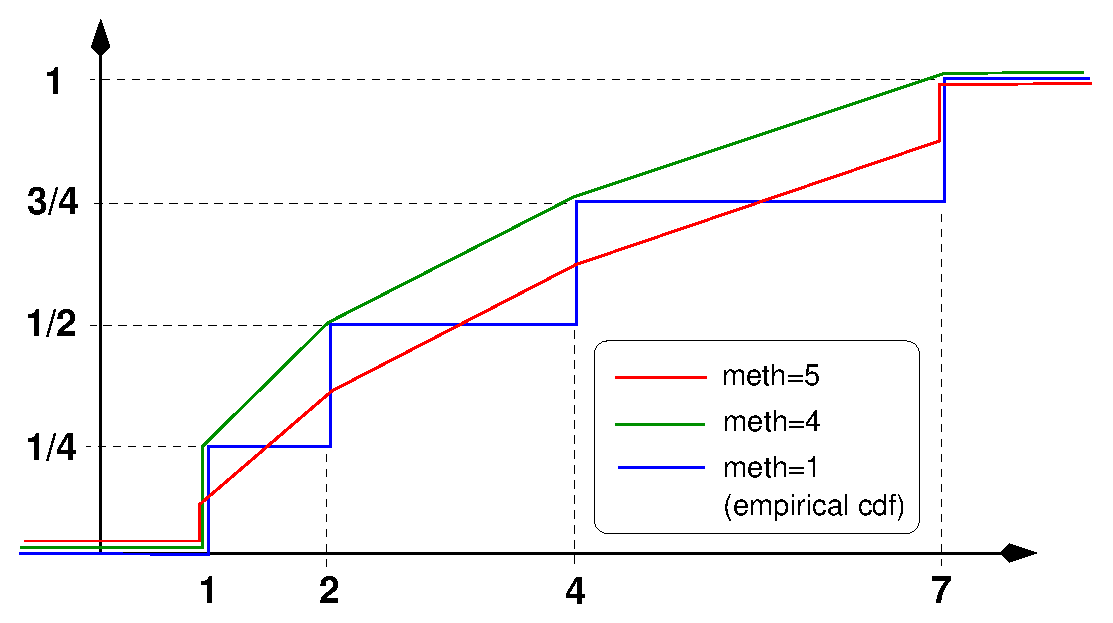
\includegraphics[width=10cm]{fctrep} 
$$



\itemdesc{meth option}

This function (which is modeled from the R and octave quantile functions) provides the 9 methods 
described in Hyndman, R.J.; Fan, Y. (November 1996). "Sample Quantiles in Statistical Packages". 
American Statistician 50 (4): 361-365. We reproduce here the explanations of the R's quantile
help page. 

All the nine sample quantiles are defined as weighted averages of consecutive order statistics
(after sorting the sample vector $X$, $x_1$ is called first order statistic, $x_2$ second order
statistic, $x_j$ $j$th  order statistic, etc...). Sample quantiles of meth $i$ are defined by:
$$
Q^{(i)}(p) = (1 - \gamma) x_j + \gamma x_{j+1}, \quad 1 \le i \le 9, \quad \frac{j-m}{n} \le p < \frac{j-m+1}{n},
$$
n is the sample size. The value of $\gamma$ is a function of $j = floor(np + m)$ and $g = np + m - j$, 
where $m$ is a constant determined by the sample quantile type. 

\begin{description}

\item[Discontinuous sample quantile methods 1, 2, and 3]

For methods 1, 2 and 3, $Q^{(meth)}$ is a discontinuous function of $p$, with $m = 0$ when $i = 1$ 
and $i = 2$, and $m = -1/2$ when $i = 3$.
\begin{itemize}
\item \itemdesc{meth=1} Inverse of empirical distribution function. $\gamma = 0$ if $g = 0$, and $1$ otherwise.

\item \itemdesc{meth=2} Similar to method $1$ but with averaging at discontinuities. $\gamma = 0.5$ if $g = 0$, and $1$ otherwise.

\item \itemdesc{meth=3} SAS definition: nearest even order statistic. $\gamma = 0$ if $g = 0$ and $j$ is even, and $1$ otherwise.
\end{itemize}

\item[~]

\item[Continuous sample quantile methods 4 through 9]

For methods 4 through 9, $Q^{(meth)}$ is a continuous function of $p$, with $\gamma = g$ and $m$ given below. 
The sample quantiles can be obtained equivalently by linear interpolation between the points 
$(p_k,x_k)$ where $x_k$ is the $k$th order statistic. Specific expressions for $p_k$ are given below. 

\begin{itemize}
\item \itemdesc{meth=4} $m=0$, $p_k = k / n$. That is, linear interpolation of the
          empirical cdf.

\item \itemdesc{meth=5} $m=1/2$, $p_k = (k - 0.5) / n$. That is a piecewise linear
          function where the knots are the values midway through the
          steps of the empirical cdf. This is used by matlab's quantile (stat toolbox), and is the default method of octave 's
          quantile, and the default for nsp).

\item \itemdesc{meth=6} $m=p$, $p_k = k / (n + 1)$. This is used by Minitab and by SPSS.

\item \itemdesc{meth=7} $m=1$, $p_k = (k - 1) / (n - 1)$. This is used by S and is the default for R.

\item \itemdesc{meth=8} $m=(p+1)/3$, $p_k = (k - 1/3) / (n + 1/3)$.  The resulting
          quantile estimates are approximately median-unbiased
          regardless of the distribution of $X$.

\item \itemdesc{meth=9} $m = p/4 + 3/8$, $p_k = (k - 3/8) / (n + 1/4)$.  The resulting
          quantile estimates are approximately unbiased for the
          expected order statistics if $X$ is normally distributed.

\end{itemize}
\end{description}

\itemdesc{dim option} 
  The dim argument (default full) gives the dimension to be used for performing the quantile 
calculations (in the following $npr$ will denote the number of components of the vector \verb+pr+):
  \begin{itemize}
    \item 'full' or 0: (default) all the elements of \verb+X+ constitute the sample. If  \verb+X+ is a row
     \verb+q+ is returned as a row vector (with $npr$ components) otherwise \verb+q+ is returned 
     as a column vector (with $npr$ components).
                       
    \item 'row' or 1: each column  of \verb+X+ is a sample ; if  \verb+X+ is an $m \times n$ array
                      so we consider $n$ samples and \verb+q+ is returned as a $npr \times n$ array.
    \item 'col' or 2: each row  of \verb+X+ is a sample ; if  \verb+X+ is an $m \times n$ array
                      so we consider $m$ samples and  \verb+q+ is returned as a $m \times npr$ array.
    \item 'm' (or -2): (for Matlab compatibility) the quantile calculations are done along the first non 
          singleton dimension of the first argument.
  \end{itemize}

\itemdesc{skip\_nan option}
   When this argument is \verb+%t+,  Nan values (which stand for ``missing or not available values'') 
 are not taking into account in the quantile computation.

\end{mandescription}
%--example 
\begin{examples}
\paragraph{example 1} sample quantiles versus exact quantiles for the Gaussian distribution
\begin{Verbatim}
n = 5000;
pr = linspace(0.01,0.99,80)';
X = randn(n,1);  // a sample from N(0,1)
q = quantile(X,pr);
qe = cdfnor("X",zeros(size(pr)),ones(size(pr)),pr,1-pr);
// compare curves
xbasc()
plot2d(pr,[q,qe],style=[2,5],leg="sample quantile@exact quantile",leg_pos="dr")
\end{Verbatim}

\paragraph{example 2} compute quartiles of a sample (and so the inter quartile range (iqr) and the median)
\begin{Verbatim}
n = 500;
X = grand(1,n,"exp",5);
pr = [0.25,0.5,0.75];
q = quantile(X,pr)
iqr = q(3) - q(1)
md = q(2)
// md should be equal to:
median(X)
\end{Verbatim}

\end{examples}

%-- see also
\begin{manseealso}
   \manlink{median}{median}, \manlink{mean}{mean}, \manlink{std}{std}
\end{manseealso}

% -- Authors
\begin{authors}
  Bruno Pincon (designed from the R's quantile help page).
\end{authors}


% -*- mode: latex -*-
\mansection{pdf}
\begin{mandesc}
  \short{pdf}{probability density functions}
\end{mandesc}
%-- Calling sequence section
\begin{calling_sequence}
\begin{verbatim}
y=pdf(dist_type, x [,p1,...,pk])  
\end{verbatim}
\end{calling_sequence}
  %-- Parameters
\begin{parameters}
  \begin{varlist}
   \vname{dist\_type}: a string given the probability distribution (\verb!"bin"!, \verb!"nor"!, \verb!"poi"!, etc ...)
    \vname{x}: scalar or vector or matrix with abscissae where the density function must be evaluated
   \vname{p1, ..., pk}: (scalar) parameters (reals or integers) required to define the distribution \verb!dist_type!
   \vname{y}: values at \verb+x+ of the given density.
  \end{varlist}
  \end{parameters}
  
\begin{mandescription}
  Computes the density function of various distributions. Most of the
  scalar probability distributions of the \manlink{grand}{grand}
  function are
  supported. 
\begin{itemize}

\item \itemdesc{beta} \verb!y=pdf(x,"bet",a,b)! computes the beta
  density with parameters $a > 0$ and $b > 0$:
$$
     f(x; a, b) =
        \frac{\Gamma(a+b)}{\Gamma(a) \Gamma(b)} x^{a-1}(1-x)^{b-1} \;
        \mbox{for } x \in (0,1)
$$

\item \itemdesc{binomial} \verb!y=pdf(x,"bin",n,p)!. Computes
  the binomial probabilities with parameters $p \in [0,1]$ and $n$
  (positive integer):
$$
     f(x; n, p) = \frac{ n! }{ x! (n-x)!} p^x (1-p)^{n-x} \;\mbox{for } x \in \{0,1,\dots,n\}
$$

\item \itemdesc{negative binomial} \verb!y=pdf(x,"bin",n,p)!. Computes
  the negative binomial probabilities with parameters $n > 0$ ($n$ not
  necessarily integer) and $p \in [0,1]$.

\item \itemdesc{Cauchy} \verb!y=pdf(x,"cau",sigma)! computes the Cauchy
  density with parameter $\sigma > 0$:
$$
     f(x; \sigma) = \frac{ \sigma }{ \pi ( x^2 + \sigma^2 ) }
$$


\item \itemdesc{chi square} \verb!y=pdf(x,"chi",nu)! computes the chi square
  density with parameter $\nu > 0$.


\item \itemdesc{exponential} \verb!y=pdf(x,"exp",tau)! computes the exponential
  density with parameter $\tau > 0$:
$$
     f(x; \tau) = \frac{1}{\tau} e^{-x/\tau} \; \mbox{for } x
     \ge 0
$$
Caution: the parameter is more frequently $\lambda = 1/\tau$.


\item \itemdesc{F variance ratio} \verb!y=pdf(x,"f",nu1,nu2)! computes
  the variance ratio density with parameters $\nu_1 > 0$ and $\nu_2 >
  0$ (respectively number of dof in the numerator and denominator).


\item \itemdesc{gamma} \verb!y=pdf(x,"gam",a,b)! computes the gamma
  density with parameters $a > 0$ (shape parameter) and $b \ge 0$
  (rate parameter):
$$
     f(x; a, b) = \frac{ b^a x^{a-1} e^{-bx} } {\Gamma(a)}\; \mbox{for } x > 0
$$
Caution: second parameter is often a scale parameter, says $s = 1/b$.

\item \itemdesc{Gauss Laplace} \verb!y=pdf(x,"nor",mu,sigma)! computes the normal
  density with parameters $\mu$ and $\sigma > 0$:
$$
     f(x; \mu, \sigma) = \frac{ 1 }{ \sigma \sqrt{2\pi}}
     e^{-\frac{1}{2} \left( \frac{x-\mu}{\sigma} \right)^2 }
$$


\item \itemdesc{geometric} \verb!y=pdf(x,"geom",p)!. Computes
  the geometric probabilities with parameter $p \in (0,1]$:
$$
     f(x; p) = (1-p)^{x-1} p \;\mbox{for } x \in \{1, 2, \dots\}
$$


\item \itemdesc{Laplace} \verb!y=pdf(x,"lap",a)! computes the Laplace
  density with parameter $a > 0$:
$$
     f(x; a) = \frac{1}{2a} e^{-\frac{|x|}{a}}
$$

\item \itemdesc{logistic} \verb!y=pdf(x,"logi",a,b)! computes the logistic
  density with parameter $a$ and $b > 0$:
$$
     f(x; a,b) = \frac{y}{b (1+y)^2}, \; \mbox{ with } y = e^{-{|x-a|}{b}}
$$


\item \itemdesc{log normal} \verb!y=pdf(x,"logn",mu,sigma)! computes
  the log normal density with parameters $\mu$ and $\sigma > 0$:
$$
     f(x; \mu, \sigma) = \frac{ 1 }{ \sigma \sqrt{2\pi}}
     e^{-\frac{1}{2} r^2 }, \; \mbox{ with } r = \frac{\log(x)-\mu}{\sigma}
$$


\item \itemdesc{Pareto} \verb!y=pdf(x,"par",a,b)! computes the Pareto
  density with parameters $a > 0$ and $b > 0$:
$$
     f(x; a, b) = \frac{ a/b }{ (x/b)^{a+1} }, \; \mbox{ for } x \ge b
$$


\item \itemdesc{Poisson} \verb!y=pdf(x,"poi",mu)!. Computes
  the Poisson probabilities with parameter $\mu \ge 0$:
$$
     f(x; \mu) = \frac{\mu^x e^{-\mu}}{x!} \;\mbox{for } x \in \{0, 1, 2, \dots\}
$$

\item \itemdesc{Rayleigh} \verb!y=pdf(x,"ray",sigma)! computes the Rayleigh
  density with parameter $\sigma > 0$:
$$
     f(x; \sigma) = \frac{x}{\sigma^2} e^{-\frac{1}{2} (x/\sigma)^2 }, \; \mbox{ for } x \ge 0
$$

\item \itemdesc{tail Rayleigh} \verb!y=pdf(x,"ray",sigma, a)! computes
  the tail Rayleigh density with parameters $\sigma > 0$ and $a \ge 0$:
$$
     f(x; \sigma, a) = \frac{x}{\sigma^2} e^{-\frac{1}{2} (x-a)(x+a)/\sigma^2 }, \; \mbox{ for } x \ge a
$$


\item \itemdesc{Weibull} \verb!y=pdf(x,"wei",a,b)! computes the Weibull
  density with parameters $a > 0$ and $b > 0$:
$$
     f(x; a, b) = \frac{b}{a} e^{ (b-1)\log(x/a) - (x/a)^b }, \; \mbox{ for } x > 0
$$

\end{itemize}

\end{mandescription}


\begin{examples}
  
\paragraph{example 1} draw N(0,1) 
\begin{program}\HCode{x = linspace(-5,5,200)';\Hnewline
y = pdf("nor",x,0,1);\Hnewline
xclear(); plot2d(x,y,style=2);\Hnewline
xtitle("The N(0,1) density function")}
\end{program}
  
\paragraph{example 2} draw Gamma(5,1) empirically (with simulation and
an histogram) and exactly (with pdf):
\begin{program}\HCode{// generate a rather big sample of Gamma(5,1) variates\Hnewline
X = grand(1e7,1,"gam",5,1);\Hnewline
// draw an histogram using 200 classes\Hnewline
xclear();histplot(200,X)\Hnewline
// superpose the exact Gamma (5,1) density\Hnewline
x = linspace(0,20,200)';\Hnewline
y = pdf("gam",x,5,1);\Hnewline
xset("thickness",2);plot2d(x,y,style=3,strf="000");xset("thickness",1)\Hnewline
xtitle("Gamma (5,1) histogram and density")}
\end{program}

\paragraph{example 3} using pdf and \verb+grand(..,"disc",..)+ to simulate
binomial random variates (when many random variates must be generated
this is faster than using directly \verb+grand(..,"bin",..)+):
\begin{program}\HCode{// compute B(500,0.3) probabilities\Hnewline
p = pdf("bin",0:500,500,0.3);\Hnewline
// now simulate B(500,0.3)\Hnewline
tic(); X = grand(1e7,1,"disc",p)-1; toc()\Hnewline
// compare with grand(..,"bin",..)\Hnewline
tic(); Y = grand(1e7,1,"bin",500,0.3); toc()\Hnewline
// display histogram for each sample and superpose exact probabilities\Hnewline
classes = (100:201 - 0.5);\Hnewline
xclear();\Hnewline
subplot(1,2,1); histplot(classes,X)\Hnewline
plot2d2(classes,p(101:201),style=5)\Hnewline
xtitle("B(500,0.3) with grand(..,""disc"",...)")\Hnewline
subplot(1,2,2); histplot(classes,Y)\Hnewline
plot2d2(classes,p(101:201),style=5)\Hnewline
xtitle("B(500,0.3) with grand(..,""bin"",...)")}
\end{program}
\end{examples}


\begin{manseealso}
  \manlink{grand}{grand}  
\end{manseealso}

%-- Authors

\begin{authors}
  beta, binomial, negative binomial, f, gamma and poisson densities uses the
  Catherine Loader 's dbinom package. Other densities and nsp interface
  Bruno Pincon.
\end{authors}


% -*- mode: latex -*-
\mansection{cdf, icdf}
\begin{mandesc}
  \short{cdf}{cumulative distribution functions} \\
  \short{icdf}{inverse cumulative distribution (aka quantile) functions} \\
\end{mandesc}
%-- Calling sequence section
\begin{calling_sequence}
\begin{verbatim}
[P,Q]=cdf(dist_type, x [,p1,...,pk])  
x=icdf(dist_type, P, [,p1,...,pk], Q=Q)
\end{verbatim}
\end{calling_sequence}
  %-- Parameters
\begin{parameters}
  \begin{varlist}
   \vname{dist\_type}: a string giving the probability distribution (\verb!"bin"! for binomial, \verb!"nor"!
   for normal, \verb!"poi"! for Poisson, etc ...)
   \vname{p1, ..., pk}: (scalar) parameters (reals or integers) required to define the distribution \verb!dist_type!
    \vname{x}: scalar or vector or matrix with abscissae where the cdf function must be evaluated or
               result for the icdf function.
   \vname{P,Q}: results of the cdf function (in this case \verb+P+ and \verb+Q+ have the same dimensions than \verb+x+)
                or inputs of the icdf function ($Q$ being given through the named optional argument \verb+Q=+)
  \end{varlist}
  \end{parameters}
  
\begin{mandescription}

For a given distribution \verb+dist_type+ and its associated parameter(s) \verb+p1, ..., pk+ :
\begin{itemize}
\item \verb![P,Q]=cdf(dist,x[,p1,...,pk])! computes the cumulative distribution function at \verb+x+, that
is if $X$ is a random variate of the given distribution :
$$
       P = F(x) := Pr ( X \le x ); \quad Q = Pr ( X > x ) = 1 - P
$$

\item and \verb!x=icdf(dist_type, P, [,p1,...,pk], Q=Q)! computes the inverse cumulative distribution function
(aka the quantile function) at \verb+P+ (\verb+Q+ can be also provided, see here after). If $F$ is the associated
cdf, its (generalized) ``inverse'' is defined by:: 
$$
\mbox{ for } P \in (0,1), \qquad   icdf(P) = F^{-1}(P) := inf \{ x \in \R : P \le F(x) \} 
$$
\end{itemize}

\paragraph{Remarks}
\begin{itemize}
\item In exact arithmetic it is equivalent to compute (for cdf) or to provide (for icdf) $P$ or $Q$ as they are
      linked by the relation $P+Q=1$ and the default is to use only $P$ ($Q$ is the second output of cdf and
      an optional input for icdf). {\bf But} as the effective computation use floating point arithmetic it 
      can be useful to compute or provide $Q$ when $P$ is near $1$ to get better accuracy (see examples).
\item When \verb+dist_type = "bet" | "bin" | "nbn" | "chi" | "nch" | "f" | "nf" | "gam" | "nor" | "poi" | "t" | "nt"+ 
      the cdf and icdf functions are just easy drivers onto the corresponding cdfxxx functions and in
      most cases :
      \begin{quote}
         \verb+[P,Q]=cdf("xxx",x,p1,..,pk)+ is equivalent to \verb+[P,Q]=cdfxxx("PQ",x,p1,..,pk)+\\
         \verb+x=icdf("xxx",P,p1,..,pk,Q=Q)+ is equivalent to \verb+x=cdfxxx("X",p1,..,pk,P,Q)+
      \end{quote}
      But note that:
      \begin{enumerate}
      \item \verb+"X"+ is not always the switch key to get the inverse cdf with the cdfxxx functions.
      \item For cdf and icdf functions the parameters p1,..,pk should be scalars while they should have
            the same dimensions than x, P, and Q for the cdfxxx functions.
      \item There are some slight differences for the icdf of discrete distributions (\verb+"bin", "nbn", "poi"+): 
            the associated cdfxxx functions (cdfbin, cdfnbn and cdfpoi) use internally a continuous extension of 
            the discrete cdf which is considered to compute the inverse cdf (but not the cdf as 
            \verb+cdfxxx("PQ",x,...)+ is applied internally on floor(x)). With the icdf function an additionnal 
            step is done to apply the definition of the generalized inverse given before and integer values are returned.
      \item The cdfxxx functions have the additionnal following feature : the value of a distribution parameter 
            can be computed when $x$ and $P$ (and the eventual  other distribution parameters) are known.
      \end{enumerate}
\end{itemize}

\paragraph{Supported distributions}
\begin{itemize}

\item \itemdesc{beta}  
\verb![P,Q]=cdf("bet",x,a,b)! and \verb!x=icdf("bet",P,a,b,Q=Q)! compute the
  cdf and icdf of the \hyperlink{betapdf}{beta distribution} with shape parameters $a > 0$ and $b > 0$.
 
\item \itemdesc{binomial}
\item \verb![P,Q]=cdf("bin",x,n,p)! and \verb!x=icdf("bin",P,n,p,Q=Q)! compute the cdf and icdf
  of the  \hyperlink{binpdf}{binomial distribution} with parameters $p \in [0,1]$ and $n$
  (positive integer). 

\item \itemdesc{negative binomial} \verb![P,Q]=cdf("nbn",x,r,p)! and \verb!x=icdf("bin",P,n,p,Q=Q)! compute
  the cdf and icdf of the \hyperlink{nbnpdf}{negative binomial distribution} with parameters $r > 0$ ($r$ not
  necessarily integer) and $p \in (0,1]$. 


\item \itemdesc{Cauchy} \verb![P,Q]=cdf("cau",x,sigma)! and  \verb!x=icdf("cau",P,sigma,Q=Q)! compute the 
  cdf and icdf of the  \hyperlink{caupdf}{Cauchy distribution} parameter $\sigma > 0$.

\item \itemdesc{chi square} \verb![P,Q]=cdf("chi",x,nu)! and  \verb!x=icdf("chi",P,nu,Q=Q)! compute the
cdf and icdf of the \hyperlink{chipdf}{chisquare distribution} with parameter $\nu > 0$ (number of dof).

\item \itemdesc{non central chi square} \verb![P,Q]=cdf("nch",x,nu,lambda)! and  \verb!x=icdf("nch",P,nu,lambda,Q=Q)! compute the
cdf and icdf of the non central chi square distribution %\hyperlink{chipdf}{chisquare distribution} 
with parameter $\nu > 0$ (number of dof) and  $\lambda > 0$ (non centrality parameter).

\item \itemdesc{exponential} \verb![P,Q]=cdf("exp",x,tau)! and \verb!x=icdf("exp",P,tau,Q=Q)! compute the cdf
and icdf of the  \hyperlink{exppdf}{exponential distribution} with parameter $\tau > 0$.
Caution: the parameter is more frequently $\lambda = 1/\tau$.

\item \itemdesc{F variance ratio} \verb![P,Q]=cdf("f",x,nu1,nu2)! and \verb!x=icdf("f",P,nu1,nu2,Q=Q)! compute
the cdf and icdf of the variance ratio distribution with parameters $\nu_1 > 0$ and $\nu_2 >
  0$ (respectively number of dof in the numerator and denominator). 

\item \itemdesc{non central F variance ratio} \verb![P,Q]=cdf("nf",x,nu1,nu2,lambda)! and \verb!x=icdf("f",P,nu1,nu2,lambda,Q=Q)! compute
the cdf and icdf of the non central F variance ratio distribution with parameters $\nu_1 > 0$, $\nu_2 > 0$ 
(respectively number of dof in the numerator and denominator) and $lambda \ge 0$ (non  centrality parameter).


\item \itemdesc{gamma} \verb![P,Q]=cdf("gam",x,a,b)! and  \verb!x=icdf("gam",P,a,b,Q=Q)! compute the cdf
 and icdf of the \hyperlink{gampdf}{gamma distribution} with parameters $a > 0$ (shape parameter) and $b \ge 0$
  (rate parameter). Caution: second parameter is often a scale parameter, says $s = 1/b$.


\item \itemdesc{Gauss Laplace} \verb![P,Q]=cdf("nor",x,mu,sigma)! and \verb!x=icdf("nor",P,mu,sigma,Q=Q)! compute
the cdf and icdf of the  \hyperlink{norpdf}{normal distribution} with parameters $\mu$ and $\sigma > 0$.


\item \itemdesc{geometric} \verb![P,Q]=cdf("geom",x,p)! and \verb!x=icdf("geom",P,p,Q=Q)! compute
the cdf and icdf of the \hyperlink{geompdf}{geometric distribution} with parameter $p \in (0,1]$.

\item \itemdesc{Kolmogorov} \verb![P,Q]=cdf("k",x,n)! computes the cdf of the Kolmogorov distribution 
with parameter $n$ (positive integer). Note that the icdf is not supported.

\item \itemdesc{limit Kolmogorov} \verb![P,Q]=cdf("klim",x)! and  \verb!x=icdf("klim",P,Q=Q)! compute the cdf 
and icdf of the limit Kolmogorov distribution (Kolmogorov distribution when $n \rightarrow \infty$). 

\item \itemdesc{Laplace} \verb![P,Q]=cdf("lap",x,a)! and \verb!x=icdf("lap",P,a,Q=Q)! compute the cdf
and icdf of the \hyperlink{lappdf}{Laplace distribution} with parameter $a > 0$.

\item \itemdesc{logistic} \verb![P,Q]=cdf("logi",x,a,b)! and \verb!x=icdf("logi",P,a,b,Q=Q)! compute the
cdf and icdf of the \hyperlink{logipdf}{logistic distribution} with parameter $a$ and $b > 0$.

\item \itemdesc{log normal} \verb![P,Q]=cdf("logn",x,mu,sigma)! and  \verb!x=icdf("logn",P,mu,sigma,Q=Q)! compute
the cdf and icdf of the  \hyperlink{lognpdf}{log normal distribution} with parameters $\mu$ and $\sigma > 0$.

\item \itemdesc{Pareto} \verb![P,Q]=cdf("par",x,a,b)! and  \verb!x=icdf("par",P,a,b,Q=Q)! compute the
cdf and icdf of the \hyperlink{parpdf}{Pareto  distribution} with shape parameter $a > 0$ and scale parameter $b > 0$.

\item \itemdesc{Poisson} \verb![P,Q]=cdf("poi",x,mu)! and \verb!x=icdf("poi",P,mu,Q=Q)! compute the
cdf and icdf of the \hyperlink{poipdf}{Poisson distribution} with parameter $\mu \ge 0$.


\item \itemdesc{Rayleigh} \verb![P,Q]=cdf("ray",x,sigma)! and \verb!x=icdf("ray",P,sigma,Q=Q)! compute
the cdf and icdf of the \hyperlink{raypdf}{Rayleigh distribution} with parameter $\sigma > 0$.

\item \itemdesc{tail Rayleigh} \verb![P,Q]=cdf("tray",x,sigma, a)! and \verb!x=icdf("tray",P,sigma,a,Q=Q)! compute
the cdf and icdf of the \hyperlink{traypdf}{tail (from $a$) of the Rayleigh distribution} with parameters $\sigma > 0$ 
and $a \ge 0$.

\item \itemdesc{Student's t} \verb![P,Q]=cdf("t",x,nu)! and \verb!x=icdf("t",P,nu,Q=Q)! compute the
cdf and icdf of the \hyperlink{tpdf}{t distribution} with parameter $\nu > 0$ (number of dof).


\item \itemdesc{non central Student's t} \verb![P,Q]=cdf("t",x,nu,delta)! and \verb!x=icdf("t",P,nu,delta,Q=Q)! compute the
cdf and icdf of the non central t distribution with parameters $\nu > 0$ (number of dof) and
$\delta$ (non centrality parameter).


\item \itemdesc{uniform (uin)} \verb![P,Q]=cdf("uin",x,n1,n2)! and \verb!x=icdf("uin",P,n1,n2,Q=Q)! compute
the cdf and icdf of the \hyperlink{uinpdf}{uniform distribution on integers $n_1,n_1+1,\dots,n_2$}.

\item \itemdesc{uniform (unf)} \verb![P,Q]=cdf("unf",x,a,b)!  and \verb!x=icdf("unf",P,a,b,Q=Q)! compute
the cdf and icdf of the \hyperlink{unfpdf}{uniform distribution on the interval $[a,b]$} ($a < b$).

\item \itemdesc{Weibull} \verb![P,Q]=cdf("wei",x,a,b)! and \verb!x=icdf("wei",P,a,b,Q=Q)! compute the
cdf and icdf of the \hyperlink{weipdf}{Weibull  distribution} with scale parameter $a > 0$ and shape parameter 
$b > 0$.

\end{itemize}

\end{mandescription}


\begin{examples}
  
\paragraph{example 1} an example with the gaussian distribution
\begin{Verbatim}
// plot pdf and cdf on [-5,5]
x = linspace(-5,5,200)';
y = pdf("nor",x,0,1);
p = cdf("nor",x,0,1);
xclear(); plot2d(x,[y,p],style=[2,5],leg="pdf@cdf");
xtitle("The N(0,1) density and cumulative distribution functions")

// apply icdf on p should return x
xx = icdf("nor",p,0,1);
max(abs(x-xx)./abs(x))  // max relative error
// if one use q, the error between x and xx should be lower
[p,q] = cdf("nor",x,0,1);
xx = icdf("nor",p,0,1,Q=q);
max(abs(x-xx)./abs(x))
\end{Verbatim}
  
\paragraph{example 2} an example with the binomial distribution
\begin{Verbatim}
n = 50; p = 0.45; // we work with Bin(n=50,p=0.45)
X = -1:n+1; Xp = nearfloat("pred",X);
x = redim([Xp;X],-1,1);
[P,Q] = cdf("bin",x,n,p);
// compare with the N(n*p,sqrt(n*p*(1-p))
mu = n*p; sigma = sqrt(n*p*(1-p));
[Pn,Qn] = cdf("nor",x,mu,sigma);
xclear(); plot2d(x,[P,Pn],style=[2,5],leg="bin@nor");
xtitle("The Bin(n,p) and N(n*p,sqrt(n*p*(1-p)) cumulative distribution functions")

// differences between icdf("bin",..) and cdfbin("S",...)
// (cdfbin use a continuous extension) 
m = 2^13+1;
P = linspace(0,1,m)';
x = icdf("bin",P,n,p);
xx = cdfbin("S",n*ones(m,1),p*ones(m,1),(1-p)*ones(m,1),P,1-P);
xclear(); plot2d(P,[x,xx],style=[2,5],leg="icdf(''bin'',..)@cdfbin(''S'',...)");
xtitle("differences between icdf(""bin"",..) and cdfbin(""S"",...)")

// with x=0:n, icdf(cdf(x)) should be equal to x
// 1/ try without using Q for icdf
x = 0:n;
[P,Q] = cdf("bin",x,n,p);
xx = icdf("bin",P,n,p);
// we don't recover x due to numerical floating point computation:
x.equal[xx]
// 2/ now use Q: we get additionnal accuracy and we recover x
xx = icdf("bin",P,n,p,Q=Q);
x.equal[xx]
\end{Verbatim}
 
\end{examples}

\begin{manseealso}
  \manlink{grand}{grand}, \manlink{pdf}{pdf}, \manlink{dist\_stat}{dist_stat}, 
  \manlink{cdfbet}{cdfbet}, \manlink{cdfbin}{cdfbin}, \manlink{cdfnbn}{cdfnbn},
  \manlink{cdfchi}{cdfchi}, \manlink{cdfchn}{cdfchn}, \manlink{cdff}{cdff}, \manlink{cdffnc}{cdffnc}, 
  \manlink{cdfgam}{cdfgam}, \manlink{cdfnor}{cdfnor}, \manlink{cdfpoi}{cdfpoi}, \manlink{cdft}{cdft}, \manlink{cdftnc}{cdftnc}.
\end{manseealso}

%-- Authors

\begin{authors}
  Buno Pincon
\end{authors}


% -*- mode: latex -*-
\mansection{dist\_stat}
\begin{mandesc}
  \short{dist_stat}{compute mean and standard deviation of some probability distributions}
\end{mandesc}
%-- Calling sequence section
\begin{calling_sequence}
\begin{verbatim}
[m,sd]=dist_stat(dist_type [,p1,...,pk])  
\end{verbatim}
\end{calling_sequence}
  %-- Parameters
\begin{parameters}
  \begin{varlist}
   \vname{dist\_type}: a string giving the probability distribution (\verb!"bin"! for binomial, \verb!"nor"!
   for normal, \verb!"poi"! for Poisson, etc ...)
   \vname{p1, ..., pk}: (scalar) parameters (reals or integers) required to define the distribution \verb!dist_type!
    \vname{m,sd}: respectively the mean and standard deviation of the selected distribution
  \end{varlist}
  \end{parameters}
  
\begin{mandescription}

For a given distribution \verb+dist_type+ and its associated parameter(s) \verb+p1, ..., pk+ this
function computes its mean and its standard deviation.

\paragraph{Supported distributions}
\begin{itemize}

\item \itemdesc{beta}  
\verb![m,sd]=dist_stat("bet",a,b)! mean and std the \hyperlink{betapdf}{beta distribution} with 
shape parameters $a > 0$ and $b > 0$.
 
\item \itemdesc{binomial}
\item \verb![m,sd]=dist_stat("bin",n,p)! mean and std
  of the  \hyperlink{binpdf}{binomial distribution} with parameters $p \in [0,1]$ and $n$
  (positive integer). 

\item \itemdesc{negative binomial} \verb![m,sd]=dist_stat("nbn",r,p)! mean and std 
of the \hyperlink{nbnpdf}{negative binomial distribution} with parameters $r > 0$ ($r$ not
  necessarily integer) and $p \in (0,1]$. 


\item \itemdesc{Cauchy} \verb![m,sd]=dist_stat("cau",sigma)! mean and std of the  
\hyperlink{caupdf}{Cauchy distribution} parameter $\sigma > 0$.

\item \itemdesc{chi square} \verb![m,sd]=dist_stat("chi",nu)! mean and std of the 
\hyperlink{chipdf}{chisquare distribution} with parameter $\nu > 0$ (number of dof).

\item \itemdesc{non central chi square} \verb![m,sd]=dist_stat("nch",nu,lambda)! mean 
nd std of the non central chi square  distribution 
%\hyperlink{chipdf}{chisquare distribution} 
with parameter $\nu > 0$ (number of dof) and  $\lambda > 0$ (non centrality parameter).

\item \itemdesc{exponential} \verb![m,sd]=dist_stat("exp",tau)! mean and std of the  
\hyperlink{exppdf}{exponential distribution} with parameter $\tau > 0$.
Caution: the parameter is more frequently $\lambda = 1/\tau$.

\item \itemdesc{F variance ratio} \verb![m,sd]=dist_stat("f",nu1,nu2)! mean and std 
of the variance ratio distribution with parameters $\nu_1 > 0$ and $\nu_2 > 0$ 
(respectively number of dof in the numerator and denominator). 

\item \itemdesc{non central F variance ratio} \verb![m,sd]=dist_stat("nf",nu1,nu2,lambda)! 
mean and std of the non central F variance ratio distribution with parameters $\nu_1 > 0$, $\nu_2 > 0$ 
(respectively number of dof in the numerator and denominator) and $lambda \ge 0$ (non  centrality parameter).


\item \itemdesc{gamma} \verb![m,sd]=dist_stat("gam",a,b)! mean and std  of the 
\hyperlink{gampdf}{gamma distribution} with parameters $a > 0$ (shape parameter) and $b \ge 0$
  (rate parameter). Caution: second parameter is often a scale parameter, says $s = 1/b$.


\item \itemdesc{Gauss Laplace} \verb![m,sd]=dist_stat("nor",mu,sigma)! mean and std 
of the  \hyperlink{norpdf}{normal distribution} with parameters $\mu$ and $\sigma > 0$.


\item \itemdesc{geometric} \verb![m,sd]=dist_stat("geom",p)! mean and std 
of the \hyperlink{geompdf}{geometric distribution} with parameter $p \in (0,1]$.


\item \itemdesc{Laplace} \verb![m,sd]=dist_stat("lap",a)! mean and std 
of the \hyperlink{lappdf}{Laplace distribution} with parameter $a > 0$.

\item \itemdesc{logistic} \verb![m,sd]=dist_stat("logi",a,b)! mean and std 
of the \hyperlink{logipdf}{logistic distribution} with parameter $a$ and $b > 0$.

\item \itemdesc{log normal} \verb![m,sd]=dist_stat("logn",mu,sigma)! mean and std 
of the  \hyperlink{lognpdf}{log normal distribution} with parameters $\mu$ and $\sigma > 0$.

\item \itemdesc{Pareto} \verb![m,sd]=dist_stat("par",a,b)! mean and std 
of the \hyperlink{parpdf}{Pareto  distribution} with shape parameter $a > 0$ and scale parameter $b > 0$.

\item \itemdesc{Poisson} \verb![m,sd]=dist_stat("poi",mu)! mean and std 
of the \hyperlink{poipdf}{Poisson distribution} with parameter $\mu \ge 0$.


\item \itemdesc{Rayleigh} \verb![m,sd]=dist_stat("ray",sigma)! mean and std 
of the \hyperlink{raypdf}{Rayleigh distribution} with parameter $\sigma > 0$.

\item \itemdesc{tail Rayleigh} \verb![m,sd]=dist_stat("tray",sigma, a)! mean and std 
of the \hyperlink{traypdf}{tail (from $a$) of the Rayleigh distribution} with parameters $\sigma > 0$ 
and $a \ge 0$.

\item \itemdesc{Student's t} \verb![m,sd]=dist_stat("t",nu)! mean and std of 
the \hyperlink{tpdf}{t distribution} with parameter $\nu > 0$ (number of dof).


\item \itemdesc{non central Student's t} \verb![m,sd]=dist_stat("nt",nu,delta)! 
mean and std of the non central t distribution with parameters $\nu > 0$ (number of dof) and
$\delta$ (non centrality parameter).


\item \itemdesc{uniform (uin)} \verb![m,sd]=dist_stat("uin",n1,n2)! mean and std 
of the \hyperlink{uinpdf}{uniform distribution on integers $n_1,n_1+1,\dots,n_2$}.

\item \itemdesc{uniform (unf)} \verb![m,sd]=dist_stat("unf",a,b)! mean and std  
of the \hyperlink{unfpdf}{uniform distribution on the interval $[a,b]$} ($a < b$).

\item \itemdesc{Weibull} \verb![m,sd]=dist_stat("wei",a,b)! mean and std of 
the \hyperlink{weipdf}{Weibull  distribution} with scale parameter $a > 0$ and shape parameter $b > 0$.

\end{itemize}

\end{mandescription}


\begin{manseealso}
  \manlink{pdf}{pdf}, \manlink{cdf}{cdf}, \manlink{icdf}{icdf}, \manlink{grand}{grand}
\end{manseealso}

%-- Authors

\begin{authors}
  Buno Pincon
\end{authors}



% -*- mode: latex -*-
\mansection{cdfbet}
\begin{mandesc}
  \short{cdfbet}{cumulative distribution function Beta distribution} 
\end{mandesc}
\index{cdfbet}\label{cdfbet}
%-- Calling sequence section
\begin{calling_sequence}
\begin{verbatim}
[P,Q]=cdfbet("PQ",X,Y,A,B)  
[X,Y]=cdfbet("XY",A,B,P,Q)  
[A]=cdfbet("A",B,P,Q,X,Y)  
[B]=cdfbet("B",P,Q,X,Y,A)  
\end{verbatim}
\end{calling_sequence}
%-- Parameters
\begin{parameters}
  \begin{varlist}
    \vname{P,Q,X,Y,A,B}: five real vectors of the same size.
    \vname{P,Q}: (\verb+Q=1-P+) the integral from 0 to X of the beta distribution (Input range: [0, 1].)
    \vname{Q}: 1-P
    \vname{X,Y}, (\verb+Y=1-X+) upper limit of integration of beta density (Input range: [0,1],  Search range: [0,1]) A,B: the two parameters of the beta density (input range: (0, +infinity), Search range: [1D-300,1D300]).
  \end{varlist}
\end{parameters}
\begin{mandescription}
  Calculates any one parameter of the beta distribution given
  values for the others. The beta density is given by
  \begin{equation}
    \frac{\Gamma(A+B)}{\Gamma(A)\Gamma(B)} x^{(A-1)} * (1-x)^{(B-1)}
  \end{equation}
  with domain $(0,1)$.
  The cumulative distribution function is calculated directly by
  code associated with the following reference: 
  DiDinato, A. R. and Morris,  A.   H.  Algorithm 708: Significant
  Digit Computation of the Incomplete  Beta  Function Ratios.  ACM
  Trans. Math.  Softw. 18 (1993), 360-373.
  Computation of other parameters involve a seach for a value that
  produces  the desired  value  of P.   The search relies  on  the
  monotinicity of P with the other parameter.
\end{mandescription}

\begin{mintednsp}{nspxxx}
x=linspace(0,1,100);
A =2;
B =3;
y= cdfbet("PQ",x,1-x,A*ones(size(x)),B*ones(size(x)));

function y=f(x)
  y = gamma(A+B)/(gamma(A)*gamma(B))*x^(A-1)*(1-x)^(B-1)
endfunction;

z=x;
for i=1:length(x)
  z(i) = intg(0,x(i),f);
end
err=max(abs(y-z));
\end{mintednsp}

\begin{authors}
  Nsp interface by Jean-Philippe Chancelier. Code from DCDFLIB: 
  Library of Fortran Routines for Cumulative Distribution
  Functions, Inverses, and Other Parameters (February, 1994)
  Barry W. Brown, James Lovato and Kathy Russell. The University of Texas.
\end{authors}


% -*- mode: latex -*-
\mansection{cdfbin}
\begin{mandesc}
  \short{cdfbin}{cumulative distribution function binomial distribution}
\end{mandesc}
\index{cdfbin}\label{cdfbin}
%-- Calling sequence section
\begin{calling_sequence}
\begin{verbatim}
[P,Q]=cdfbin("PQ",S,Xn,Pr,Ompr)      // compute cdf
[S]=cdfbin("S",Xn,Pr,Ompr,P,Q)       // compute inverse cdf (quantile function)
[Xn]=cdfbin("Xn",Pr,Ompr,P,Q,S)      // compute Xn parameter
[Pr,Ompr]=cdfbin("PrOmpr",P,Q,S,Xn)  // compute Pr and Ompr parameter
\end{verbatim}
\end{calling_sequence}
%-- Parameters
\begin{parameters}
  \begin{varlist}
    \vname{P,Q,S,Xn,Pr,Ompr}: six real vectors of the same size.
    \vname{P,Q (Q=1-P)}: the cumulation from 0 to S of the binomial distribution. (Probability of S or fewer successes in Xn trials each with probability of success Pr.) Input range: [0,1].
    \vname{S}: the number of successes observed. Search range: [0, XN]
    \vname{Xn}: the number of binomial trials. Input range: (0, +infinity). Search range: [1E-300, 1E300]
    \vname{Pr,Ompr (Ompr=1-Pr)}: the probability of success in each binomial trial. Input range: [0,1]. Search range: [1E-300,1]
  \end{varlist}
\end{parameters}

\begin{mandescription}
  Calculates any one parameter of the binomial distribution given values 
  for the others. Formula  26.5.24 of  Abramowitz and Stegun,  Handbook   of
  Mathematical   Functions (1966) is used  to reduce the  binomial
  distribution  to  the  cumulative beta distribution.
  Computation of other parameters involve a search for a value that
  produces  the desired  value  of P.
\end{mandescription}

\begin{examples}
\begin{mintednsp}{nsp}
// compute then display the cumulative distribution function
Xn = 18; pr = 0.45;
x = 0:Xn+1; xp = nearfloat("pred",x);
x = [xp;x]; x.redim[-1,1]; 
v = ones(size(x));
P=cdfbin("PQ",x,Xn*v,pr*v,(1-pr)*v); // you can use cdf("bin",x,Xn,pr)
xbasc()
plot2d(x,P,style=2,leg="cdf(x)")
\end{mintednsp}
\end{examples}

\begin{authors}
  Nsp interface by Jean-Philippe Chancelier. Fortran code from DCDFLIB
  adapted in C and improved/modified by Bruno Pincon and Jean-Philippe Chancelier.  
  DCDFLIB: Library of Fortran Routines for Cumulative Distribution
  Functions, Inverses, and Other Parameters (February, 1994)
  Barry W. Brown, James Lovato and Kathy Russell. The University of Texas.
\end{authors}


% -*- mode: latex -*-
\mansection{cdfchi}
\begin{mandesc}
  \short{cdfchi}{cumulative distribution function chi-square distribution}
\end{mandesc}
\index{cdfchi}\label{cdfchi}
%-- Calling sequence section
\begin{calling_sequence}
\begin{verbatim}
  [P,Q]=cdfchi("PQ",X,Df)  
  [X]=cdfchi("X",Df,P,Q);  
  [Df]=cdfchi("Df",P,Q,X)  
\end{verbatim}
\end{calling_sequence}
%-- Parameters
\begin{parameters}
  \begin{varlist}
    \vname{P,Q,Xn,Df}: four real vectors of the same size.
    \vname{P,Q (Q=1-P)}:  the integral from 0 to X of the chi-square distribution. Input range: [0, 1]. 
    \vname{X}: upper limit of integration of the non-central chi-square distribution. Input range: [0, +infinity). Search range: [0,1E300]  
      \vname{Df}: degrees of freedom of the chi-square distribution. Input range: (0, +infinity). Search range: [ 1E-300, 1E300]
  \end{varlist}
\end{parameters}
\begin{mandescription}
  Calculates any one parameter of the chi-square 
  distribution given values for the others.
  The chi-square distribution is given by:
  \begin{equation}
    \frac{(1/2)^{(Df/2)}}{\Gamma(Df/2)} x^{(Df/2 -1)} * e^{-x/2} 
  \end{equation}
  with domain $(0,\infty)$.
  Formula    26.4.19   of Abramowitz  and     Stegun, Handbook  of
  Mathematical Functions   (1966) is used   to reduce the chi-square
  distribution to the incomplete distribution.
  Computation of other parameters involve a seach for a value that
  produces  the desired  value  of P.   The search relies  on  the
  monotinicity of P with the other parameter.
\end{mandescription}

\begin{authors}
  Nsp interface by Jean-Philippe Chancelier. Code from DCDFLIB: 
  Library of Fortran Routines for Cumulative Distribution
  Functions, Inverses, and Other Parameters (February, 1994)
  Barry W. Brown, James Lovato and Kathy Russell. The University of Texas.
\end{authors}

% -*- mode: latex -*-
\mansection{cdfchn}
\begin{mandesc}
  \short{cdfchn}{cumulative distribution function  non-central chi-square distribution}
\end{mandesc}
\index{cdfchn}\label{cdfchn}
%-- Calling sequence section
\begin{calling_sequence}
\begin{verbatim}
  [P,Q]=cdfchn("PQ",X,Df,Pnonc)  
  [X]=cdfchn("X",Df,Pnonc,P,Q);  
  [Df]=cdfchn("Df",Pnonc,P,Q,X)  
  [Pnonc]=cdfchn("Pnonc",P,Q,X,Df)  
\end{verbatim}
\end{calling_sequence}
%-- Parameters
\begin{parameters}
  \begin{varlist}
    \vname{P,Q,X,Df,Pnonc}: five real vectors of the same size.
    \vname{P,Q (Q=1-P)}:  the integral from 0 to X of the non-central chi-square distribution. 
    Input range: [0, 1-1E-16).
      \vname{X}: upper limit of integration of the non-central chi-square distribution. Input range: [0, +infinity). Search range: [0,1E300]
        \vname{Df}: degrees of freedom of the non-central chi-square distribution. Input range: (0, +infinity). Search range: [ 1E-300, 1E300]
        \vname{Pnonc}:  non-centrality parameter of the non-central chi-square distribution. Input range: [0, +infinity). Search range: [0,1E4]
  \end{varlist}
\end{parameters}

\begin{mandescription}
  Calculates any one parameter of the non-central chi-square
  distribution given values for the others. Let $\lambda = \mbox{Pnonc}$ and 
  $k = \mbox{Df}$ the probability density function of the noncentral chi-square 
  distribution is given for $x\in [0,\infty)$  by~:
  \begin{equation} 
    \frac{1}{2}e^{-(x+\lambda)/2}\left (\frac{x}{\lambda} \right)^{k/4-1/2} I_{k/2-1}(\sqrt{\lambda x})
  \end{equation}
  where $I_a(x)$ is a modified Bessel function of the first kind given by~:
  \begin{equation} 
      I_a(y) = (y/2)^a \sum_{j=0}^\infty \frac{ (y^2/4)^j}{j! \Gamma(a+j+1)} 
  \end{equation}
  Formula  26.4.25 of Abramowitz and Stegun,
  Handbook  of Mathematical  Functions (1966) is used to compute the cumulative
  distribution function.
  Computation of other parameters involve a seach for a value that
  produces  the desired  value  of P.   The search relies  on  the
  monotinicity of P with the other parameter.
  The computation time  required for this  routine is proportional
  to the noncentrality  parameter  (PNONC).  Very large  values of
  this parameter can consume immense  computer resources.  This is
  why the search range is bounded by $10^4$.
\end{mandescription}

\begin{authors}
  Nsp interface by Jean-Philippe Chancelier. Code from DCDFLIB: 
  Library of Fortran Routines for Cumulative Distribution
  Functions, Inverses, and Other Parameters (February, 1994)
  Barry W. Brown, James Lovato and Kathy Russell. The University of Texas.
\end{authors}

% -*- mode: latex -*-

\mansection{cdff}
\begin{mandesc}
  \short{cdff}{cumulative distribution function F distribution}
\end{mandesc}
\index{cdff}\label{cdff}
%-- Calling sequence section
\begin{calling_sequence}
\begin{verbatim}
  [P,Q]=cdff("PQ",F,Dfn,Dfd)  
  [F]=cdff("F",Dfn,Dfd,P,Q);  
  [Dfn]=cdff("Dfn",Dfd,P,Q,F);  
  [Dfd]=cdff("Dfd",P,Q,F,Dfn)  
\end{verbatim}
\end{calling_sequence}
%-- Parameters
\begin{parameters}
  \begin{varlist}
    \vname{P,Q,F,Dfn,Dfd}: five real vectors of the same size.
    \vname{P,Q (Q=1-P)}:  the integral from 0 to F of the f-density. Input range: [0,1].
    \vname{F}: upper limit of integration of the f-density. Input range: [0, +infinity). Search range: [0,1E300]
      \vname{Dfn}: degrees of freedom of the numerator sum of squares. Input range: (0, +infinity). Search range: [ 1E-300, 1E300]
      \vname{Dfd}: degrees of freedom of the denominator sum of squares. Input range: (0, +infinity). Search range: [ 1E-300, 1E300]
  \end{varlist}
\end{parameters}
\begin{mandescription}
  Calculates any one parameter of the F distribution
  given values for the others.
  Formula   26.6.2   of   Abramowitz   and   Stegun,  Handbook  of
  Mathematical  Functions (1966) is used to reduce the computation
  of the  cumulative  distribution function for the  F  variate to
  that of an incomplete beta.
  Computation of other parameters involve a seach for a value that
  produces  the desired  value  of P.   The search relies  on  the
  monotinicity of P with the other parameter.
  The value of the  cumulative  F distribution is  not necessarily
  monotone in  either degrees of freedom.  There  thus may  be two
  values  that  provide a given CDF  value.   This routine assumes
  monotonicity and will find an arbitrary one of the two values.
\end{mandescription}

\begin{authors}
  Nsp interface by Jean-Philippe Chancelier. Code from DCDFLIB: 
  Library of Fortran Routines for Cumulative Distribution
  Functions, Inverses, and Other Parameters (February, 1994)
  Barry W. Brown, James Lovato and Kathy Russell. The University of Texas.
\end{authors}

% -*- mode: latex -*-
\mansection{cdffnc}
\begin{mandesc}
  \short{cdffnc}{cumulative distribution function non-central f-distribution}
\end{mandesc}
\index{cdffnc}\label{cdffnc}
%-- Calling sequence section
\begin{calling_sequence}
\begin{verbatim}
  [P,Q]=cdffnc("PQ",F,Dfn,Dfd,Pnonc)  
  [F]=cdffnc("F",Dfn,Dfd,Pnonc,P,Q);  
  [Dfn]=cdffnc("Dfn",Dfd,Pnonc,P,Q,F);  
  [Dfd]=cdffnc("Dfd",Pnonc,P,Q,F,Dfn)  
  [Pnonc]=cdffnc("Pnonc",P,Q,F,Dfn,Dfd);  
\end{verbatim}
\end{calling_sequence}
%-- Parameters
\begin{parameters}
  \begin{varlist}
    \vname{P,Q,F,Dfn,Dfd,Pnonc}: six real vectors of the same size.
    \vname{P,Q (Q=1-P)} the integral from 0 to F of the non-central f-density. Input range: [0,1-1E-16).
      \vname{F}: upper limit of integration of the non-central f-density. Input range: [0, +infinity). Search range: [0,1E300]
        \vname{Dfn}: degrees of freedom of the numerator sum of squares. Input range: (0, +infinity). Search range: [ 1E-300, 1E300]
        \vname{Dfd}: degrees of freedom of the denominator sum of squares. Must be in range: (0, +infinity). Input range: (0, +infinity). Search range: [ 1E-300, 1E300]
        \vname{Pnonc}: the non-centrality parameter Input range: [0,infinity) Search range: [0,1E4]
  \end{varlist}
\end{parameters}
\begin{mandescription}
  Calculates any one parameter of the Non-central F distribution given values for the others.

  Formula  26.6.20   of   Abramowitz   and   Stegun,  Handbook  of
  Mathematical  Functions (1966) is used to compute the cumulative
  distribution function.
  Computation of other parameters involve a seach for a value that
  produces  the desired  value  of P.   The search relies  on  the
  monotinicity of P with the other parameter.
  The computation time  required for this  routine is proportional
  to the noncentrality  parameter  (PNONC).  Very large  values of
  this parameter can consume immense  computer resources.  This is
  why the search range is bounded by 10,000.
  The  value  of the  cumulative  noncentral F distribution is not
  necessarily monotone in either degrees  of freedom.  There  thus
  may be two values that provide a given  CDF value.  This routine
  assumes monotonicity  and will find  an arbitrary one of the two
  values.
\end{mandescription}

\begin{authors}
  Nsp interface by Jean-Philippe Chancelier. Code from DCDFLIB: 
  Library of Fortran Routines for Cumulative Distribution
  Functions, Inverses, and Other Parameters (February, 1994)
  Barry W. Brown, James Lovato and Kathy Russell. The University of Texas.
\end{authors}

% -*- mode: latex -*-
\mansection{cdfgam}
\begin{mandesc}
  \short{cdfgam}{cumulative distribution function gamma distribution}
\end{mandesc}
\index{cdfgam}\label{cdfgam}
  %-- Calling sequence section
\begin{calling_sequence}
\begin{verbatim}
[P,Q]=cdfgam("PQ",X,Shape,Rate)  
[X]=cdfgam("X",Shape,Rate,P,Q)  
[Shape]=cdfgam("Shape",Rate,P,Q,X)  
[Rate]=cdfgam("Rate",P,Q,X,Shape)  
\end{verbatim}
\end{calling_sequence}
%-- Parameters
\begin{parameters}
  \begin{varlist}
    \vname{P,Q,X,Shape,Rate}: five real vectors of the same size.
    \vname{P,Q (Q=1-P)} the integral from 0 to X of the gamma density. Input range: [0,1].
    \vname{X}:  the upper limit of integration of the gamma density. Input range: [0, +infinity). Search range: [0,1E300]
      \vname{Shape}:  the shape parameter of the gamma density. Input range: (0, +infinity). Search range: [1E-300,1E300]
      \vname{Rate}:  the scale parameter of the gamma density. Input range: (0, +infinity). Search range: (1E-300,1E300]
  \end{varlist}
\end{parameters}
\begin{mandescription}
  Calculates any one parameter of the gamma distribution given values for the others.
  The gamma density is given by for $x>0$ by~:
  \begin{equation}
    x^{\alpha-1} \frac{ \beta^\alpha  e^{- \beta x}}{\Gamma(\alpha)}
  \end{equation}
  where $\alpha = \mbox{\tt Shape}$ and $\beta = \mbox{\tt Rate}$. 
  Note that usually the second parameter of the gamma distribution 
  is a \verb!Scale! parameter equal to the inverse of the \verb!Rate! 
  (so you have to use \verb!Rate = 1/Shape!).

  Cumulative distribution function (P) is calculated directly by
  the code associated with: DiDinato, A. R. and Morris, A. H. 
  Computation of the  incomplete
  gamma function  ratios  and their  inverse.   ACM  Trans.  Math.
  Softw. 12 (1986), 377-393.
  Computation of other parameters involve a seach for a value that
  produces  the desired  value  of P.   The search relies  on  the
  monotinicity of P with the other parameter.
\end{mandescription}

\begin{program}\HCode{x=linspace(0,20,100);\Hnewline
shape =1;\Hnewline
scale =0.5;\Hnewline
y= cdfgam("PQ",x,shape*ones(x),scale*ones(x));\Hnewline
\Hnewline
function y=f(x)\Hnewline
  y = x^(shape-1)*scale^shape*exp(-x*scale)./gamma(shape);\Hnewline
endfunction;\Hnewline
\Hnewline
z=x;\Hnewline
for i=1:length(x)\Hnewline
  z(i) = intg(0,x(i),f);\Hnewline
end\Hnewline
err=max(abs(y-z));}
\end{program}

\begin{authors}
  Nsp interface by Jean-Philippe Chancelier. Code from DCDFLIB: 
  Library of Fortran Routines for Cumulative Distribution
  Functions, Inverses, and Other Parameters (February, 1994)
  Barry W. Brown, James Lovato and Kathy Russell. The University of Texas.
\end{authors}

% -*- mode: latex -*-
\mansection{cdfnbn}
\begin{mandesc}
  \short{cdfnbn}{cumulative distribution function  negative binomial distribution}
\end{mandesc}
\index{cdfnbn}\label{cdfnbn}
%-- Calling sequence section
\begin{calling_sequence}
\begin{verbatim}
  [P,Q]=cdfnbn("PQ",S,Xn,Pr,Ompr)  
  [S]=cdfnbn("S",Xn,Pr,Ompr,P,Q)  
  [Xn]=cdfnbn("Xn",Pr,Ompr,P,Q,S)  
  [Pr,Ompr]=cdfnbn("PrOmpr",P,Q,S,Xn)  
\end{verbatim}
\end{calling_sequence}
%-- Parameters
\begin{parameters}
  \begin{varlist}
    \vname{P,Q,S,Xn,Pr,Ompr}: six real vectors of the same size.
    \vname{P,Q (Q=1-P)}: the cumulation from 0 to S of the  negative binomial distribution. Input range: [0,1].
    \vname{S}: the upper limit of cumulation of the binomial distribution. There are F or fewer failures before the XNth success. Input range: [0, +infinity). Search range: [0, 1E300]
      \vname{Xn}: the number of successes. Input range: [0, +infinity). Search range: [0, 1E300]
        \vname{Pr}:  the probability of success in each binomial trial. Input range: [0,1]. Search range: [0,1].
        \vname{Ompr}:  \verb+1-PR+ Input range: [0,1]. Search range: [0,1]. \verb+PR + OMPR = 1.0+.
  \end{varlist}
\end{parameters}
\begin{mandescription}
  Calculates any one parameter of the negative binomial
  distribution given values for the others.
  The  cumulative  negative   binomial  distribution  returns  the
  probability that there  will be  F or fewer failures before  the
  XNth success in binomial trials each of which has probability of
  success PR.
  The individual term of the negative binomial is the probability of
  S failures before XN successes and is
  Choose \verb!( S, XN+S-1 ) * PR^(XN) * (1-PR)^S!
  Formula   26.5.26   of   Abramowitz  and  Stegun,  Handbook   of
  Mathematical Functions (1966) is used  to  reduce calculation of
  the cumulative distribution  function to that of  an  incomplete
  beta.
  Computation of other parameters involve a seach for a value that
  produces  the desired  value  of P.   The search relies  on  the
  monotinicity of P with the other parameter.
\end{mandescription}

\begin{authors}
  Nsp interface by Jean-Philippe Chancelier. Code from DCDFLIB: 
  Library of Fortran Routines for Cumulative Distribution
  Functions, Inverses, and Other Parameters (February, 1994)
  Barry W. Brown, James Lovato and Kathy Russell. The University of Texas.
\end{authors}

% -*- mode: latex -*-
\mansection{cdfnor}
\begin{mandesc}
  \short{cdfnor}{cumulative distribution function normal distribution}
\end{mandesc}
\index{cdfnor}\label{cdfnor}
%-- Calling sequence section
\begin{calling_sequence}
\begin{verbatim}
  [P,Q]=cdfnor("PQ",X,Mean,Std)  
  [X]=cdfnor("X",Mean,Std,P,Q)  
  [Mean]=cdfnor("Mean",Std,P,Q,X)  
  [Std]=cdfnor("Std",P,Q,X,Mean)  
\end{verbatim}
\end{calling_sequence}
%-- Parameters
\begin{parameters}
  \begin{varlist}
    \vname{P,Q,X,Mean,Std}: six real vectors of the same size.
    \vname{P,Q (Q=1-P)}: the integral from -infinity to X of the normal density. Input range: (0,1].
      \vname{X}: upper limit of integration of the normal-density. Input range: ( -infinity, +infinity)
      \vname{Mean}: the mean of the normal density. Input range: (-infinity, +infinity)
      \vname{Sd}: standard Deviation of the normal density. Input range: (0, +infinity).
  \end{varlist}
\end{parameters}
\begin{mandescription}
  Calculates any one parameter of the normal distribution given values for the others.
  The normal density is given by~:
  \begin{equation}
    \frac{1}{\sigma\sqrt{2\pi}} \; \exp\left(-\frac{\left(x-\mu\right)^2}{2\sigma^2} \right)
  \end{equation} 
  with $\sigma = \mbox{\tt Std}$ and $\mu = \mbox{\tt Mean}$.
  The  cumulative standard normal distribution is computed with a C rewriten version of 
  anorm from W.D Cody (1993) ("ALGORITHM 715: SPECFUN - A Portable FORTRAN
  Package of Special Function Routines and Test Drivers" ACM Transactions on Mathematical Software. 19, 22-32) 

  The rational functions from pages  90-95  of Kennedy and Gentle,
  Statistical  Computing,  Marcel  Dekker, NY,  1980 are  used  as
  starting values to Newton's Iterations which compute the inverse
  standard normal.  Therefore no  searches  are necessary for  any
  parameter. 
  For X $<$ -15, the asymptotic expansion for the normal is used  as
  the starting value in finding the inverse standard normal.
  This is formula 26.2.12 of Abramowitz and Stegun.
\end{mandescription}

\begin{program}\HCode{x=linspace(-5,5,100);\Hnewline
mu =1;\Hnewline
sig =0.5;\Hnewline
y= cdfnor("PQ",x,mu*ones(x),sig*ones(x));\Hnewline
\Hnewline
function y=f(x)\Hnewline
  y= (1/2)*(1 + erf((x-mu)/(sig*sqrt(2))));\Hnewline
endfunction;\Hnewline
\Hnewline
z=f(x);\Hnewline
err=max(abs(y-z));}
\end{program}

\begin{authors}
  Nsp interface by Jean-Philippe Chancelier. Code from DCDFLIB: 
  Library of Fortran Routines for Cumulative Distribution
  Functions, Inverses, and Other Parameters (February, 1994)
  Barry W. Brown, James Lovato and Kathy Russell. The University of Texas.
\end{authors}

% -*- mode: latex -*-
\mansection{cdfpoi}
\begin{mandesc}
  \short{cdfpoi}{cumulative distribution function poisson distribution}
\end{mandesc}
\index{cdfpoi}\label{cdfpoi}
%-- Calling sequence section
\begin{calling_sequence}
\begin{verbatim}
  [P,Q]=cdfpoi("PQ",S,Xlam)  
  [S]=cdfpoi("S",Xlam,P,Q)  
  [Xlam]=cdfpoi("Xlam",P,Q,S);  
\end{verbatim}
\end{calling_sequence}
%-- Parameters
\begin{parameters}
  \begin{varlist}
    \vname{P,Q,S,Xlam} : four real vectors of the same size.
    \vname{P,Q (Q=1-P)  } :  The cumulation from 0 to S of the poisson density. Input range: [0,1].
    \vname{S} :Upper limit of cumulation of the Poisson. Input range: [0, +infinity). Search range: [0,1E300]
      \vname{Xlam} :  Mean of the Poisson distribution. Input range: [0, +infinity). Search range: [0,1E300]
  \end{varlist}
\end{parameters}
\begin{mandescription}
  Calculates any one parameter of the Poisson
  distribution given values for the others.
  Formula   26.4.21  of   Abramowitz  and   Stegun,   Handbook  of
  Mathematical Functions (1966) is used  to reduce the computation
  of  the cumulative distribution function to that  of computing a
  chi-square, hence an incomplete gamma function.
  Cumulative  distribution function  (P) is  calculated  directly.
  Computation of other parameters involve a seach for a value that
  produces  the desired value of  P.   The  search relies  on  the
  monotinicity of P with the other parameter.
\end{mandescription}

\begin{authors}
  Nsp interface by Jean-Philippe Chancelier. Code from DCDFLIB: 
  Library of Fortran Routines for Cumulative Distribution
  Functions, Inverses, and Other Parameters (February, 1994)
  Barry W. Brown, James Lovato and Kathy Russell. The University of Texas.
\end{authors}

% -*- mode: latex -*-
\mansection{cdft}
\begin{mandesc}
  \short{cdft}{cumulative distribution function Student's T distribution}
\end{mandesc}
\index{cdft}\label{cdft}
%-- Calling sequence section
\begin{calling_sequence}
\begin{verbatim}
  [P,Q]=cdft("PQ",T,Df)  
  [T]=cdft("T",Df,P,Q)  
  [Df]=cdft("Df",P,Q,T)  
\end{verbatim}
\end{calling_sequence}
%-- Parameters
\begin{parameters}
  \begin{varlist}
    \vname{P,Q,T,Df}: six real vectors of the same size.
    \vname{P,Q (Q=1-P)}: the integral from -infinity to t of the t-density. Input range: (0,1].
      \vname{T}: upper limit of integration of the t-density. Input range: ( -infinity, +infinity). Search range: [ -1E150, 1E150 ]
      \vname{DF:} degrees of freedom of the t-distribution. Input range: (0 , +infinity). Search range: [1e-300, 1E10]
  \end{varlist}
\end{parameters}
\begin{mandescription}
  Calculates any one parameter of the T distribution given
  values for the others. The T distribution is given by~:
  \begin{equation}
    \frac{\Gamma(\frac{\nu+1}{2})} {\sqrt{\nu\pi}\,\Gamma(\frac{\nu}{2})} \left(1+\frac{t^2}{\nu} \right)^{-(\frac{\nu+1}{2})} 
  \end{equation}
  with $\nu = \mbox{\tt Df}$  and where $\Gamma$ is the Gamma function.
  Formula  26.5.27  of   Abramowitz   and  Stegun,   Handbook   of
  Mathematical Functions  (1966) is used to reduce the computation
  of the cumulative distribution function to that of an incomplete
  beta.
  Computation of other parameters involve a seach for a value that
  produces  the desired  value  of P.   The search relies  on  the
  monotinicity of P with the other parameter.
\end{mandescription}

\begin{program}\HCode{x=linspace(-10,10,100);\Hnewline
df = 3;\Hnewline
y= cdft("PQ",x,df*ones(x));\Hnewline
function y=f(x)\Hnewline
  y = gamma((df+1)/2)/( sqrt(df*\%pi) *gamma(df/2))*(1+x^2/df)^(-(df+1)/2);\Hnewline
endfunction;\Hnewline
\Hnewline
z=x;\Hnewline
for i=1:length(x)\Hnewline
  z(i) = intg(-1000,x(i),f);\Hnewline
end\Hnewline
err=max(abs(y-z));}
\end{program}


\begin{authors}
  Nsp interface by Jean-Philippe Chancelier. Code from DCDFLIB: 
  Library of Fortran Routines for Cumulative Distribution
  Functions, Inverses, and Other Parameters (February, 1994)
  Barry W. Brown, James Lovato and Kathy Russell. The University of Texas.
\end{authors}

% -*- mode: latex -*-
\mansection{cdft}
\begin{mandesc}
  \short{cdftnc}{cumulative distribution function Student's non-central T distribution}
\end{mandesc}
\index{cdft}\label{cdft}
%-- Calling sequence section
\begin{calling_sequence}
\begin{verbatim}
  [P,Q]=cdft("PQ",T,Df,Pnonc)  
  [T]=cdft("T",Df,Pnonc,P,Q)  
  [Df]=cdft("Df",Pnonc,P,Q,T)  
\end{verbatim}
\end{calling_sequence}
%-- Parameters
\begin{parameters}
  \begin{varlist}
    \vname{P,Q,T,Df,PNONC} : six real vectors of the same size.
    \vname{P,Q (Q=1-P)  } : The integral from -infinity to t of the t-density. Input range: (0,1].
      \vname{T} : Upper limit of integration of the t-density. Input range: ( -infinity, +infinity). Search range: [ -1E150, 1E150 ]
      \vname{DF:  } Degrees of freedom of the t-distribution. Input range: (0 , +infinity). Search range: [1e-300, 1E10]
  \end{varlist}
\end{parameters}
\begin{mandescription}
  Calculates any one parameter of the non-central T distribution given
  values for the others.
  Upper tail    of  the  cumulative  noncentral t is calculated using 
  formulae  from page 532  of Johnson, Kotz,  Balakrishnan, Coninuous 
  Univariate Distributions, Vol 2, 2nd Edition.  Wiley (1995) 
  Computation of other parameters involve a seach for a value that 
  produces  the desired  value  of P.   The search relies  on  the 
  monotinicity of P with the other parameter. 
\end{mandescription}

\begin{authors}
  Nsp interface by Jean-Philippe Chancelier. Code from DCDFLIB: 
  Library of Fortran Routines for Cumulative Distribution
  Functions, Inverses, and Other Parameters (February, 1994)
  Barry W. Brown, James Lovato and Kathy Russell. The University of Texas.
\end{authors}

